\documentclass[a4paper,12pt]{article}
\usepackage[T1]{fontenc}
\usepackage{times}
\usepackage[english]{babel}
\usepackage[utf8]{inputenc}
\usepackage{dtklogos}
\usepackage{subcaption}
\usepackage{listings}
\usepackage{amssymb}
\usepackage{float}
\usepackage{wallpaper}
\usepackage[absolute]{textpos}
\usepackage[top=2cm, bottom=2.5cm, left=3cm, right=3cm]{geometry}
\usepackage{appendix}
\usepackage[colorlinks=true, linkcolor=black, urlcolor=blue, citecolor=black]{hyperref}
\colorlet{punct}{red!60!black}
\definecolor{background}{HTML}{EEEEEE}
\definecolor{delim}{RGB}{20,105,176}
\colorlet{numb}{magenta!60!black}
\lstdefinelanguage{json}{
    basicstyle=\fontsize{9pt}{9pt}\ttfamily,
    numbers=left,
    numberstyle=\scriptsize,
    stepnumber=0,
    numbersep=0pt,
    tabsize=4,
    showstringspaces=false,
    breaklines=true,
    frame=lines,
    backgroundcolor=\color{background},
    literate=
     *{0}{{{\color{numb}0}}}{1}
      {1}{{{\color{numb}1}}}{1}
      {2}{{{\color{numb}2}}}{1}
      {3}{{{\color{numb}3}}}{1}
      {4}{{{\color{numb}4}}}{1}
      {5}{{{\color{numb}5}}}{1}
      {6}{{{\color{numb}6}}}{1}
      {7}{{{\color{numb}7}}}{1}
      {8}{{{\color{numb}8}}}{1}
      {9}{{{\color{numb}9}}}{1}
      {:}{{{\color{punct}{:}}}}{1}
      {,}{{{\color{punct}{,}}}}{1}
      {\{}{{{\color{delim}{\{}}}}{1}
      {\}}{{{\color{delim}{\}}}}}{1}
      {[}{{{\color{delim}{[}}}}{1}
      {]}{{{\color{delim}{]}}}}{1},
}
\setcounter{secnumdepth}{4}
\setcounter{tocdepth}{4}
\usepackage{sectsty}
\sectionfont{\fontsize{14}{15}\selectfont}
\subsectionfont{\fontsize{12}{15}\selectfont}
\subsubsectionfont{\fontsize{12}{15}\selectfont}
\usepackage{csquotes} 
\renewcommand{\thetable}{\arabic{section}.\arabic{table}}  
\renewcommand{\thefigure}{\arabic{section}.\arabic{figure}}
\newsavebox{\mybox}
\newlength{\mydepth}
\newlength{\myheight}
\newenvironment{sidebar}
{\begin{lrbox}{\mybox}\begin{minipage}{\textwidth}}
{\end{minipage}\end{lrbox}
 \settodepth{\mydepth}{\usebox{\mybox}}
 \settoheight{\myheight}{\usebox{\mybox}}
 \addtolength{\myheight}{\mydepth}
 \noindent\makebox[0pt]{\hspace{-20pt}\rule[-\mydepth]{1pt}{\myheight}}%
 \usebox{\mybox}}
\newcommand\BackgroundPic{
    \put(-2,-3){
    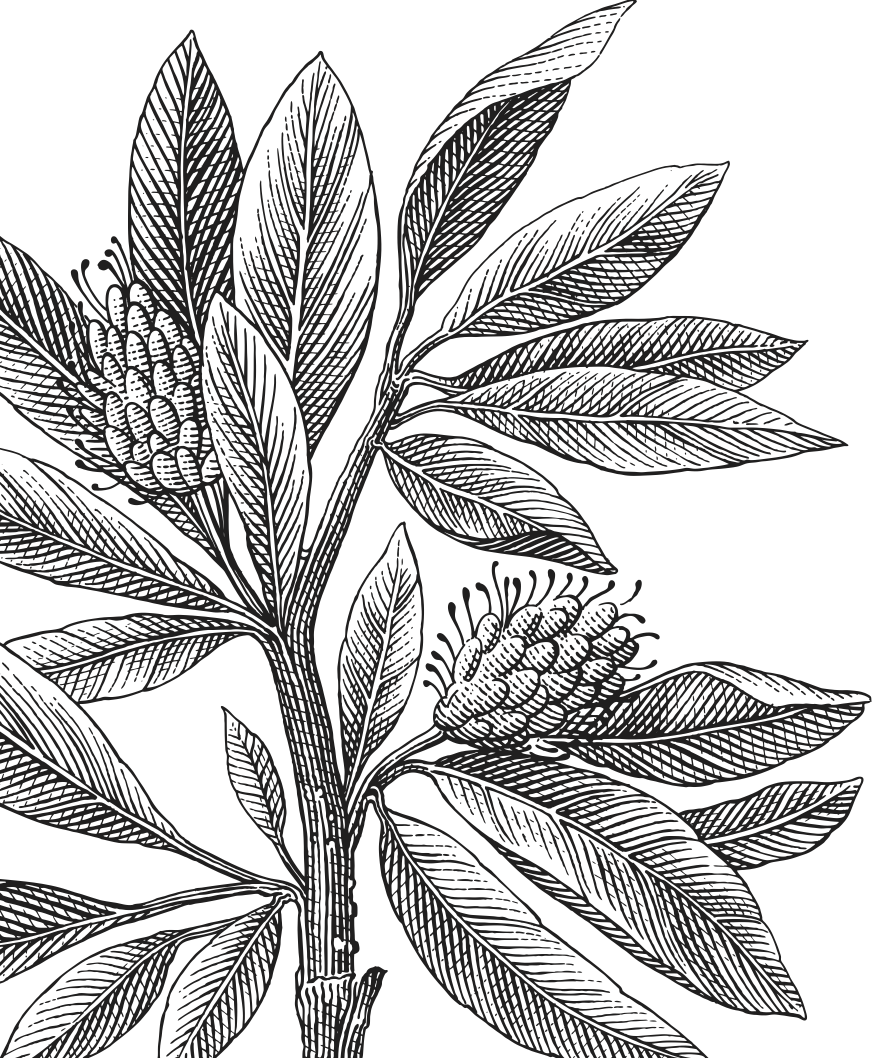
\includegraphics[keepaspectratio,scale=0.3]{figures/lnu_etch.png}
    }
}
\newcommand\BackgroundPicLogo{
    \put(30,740){
    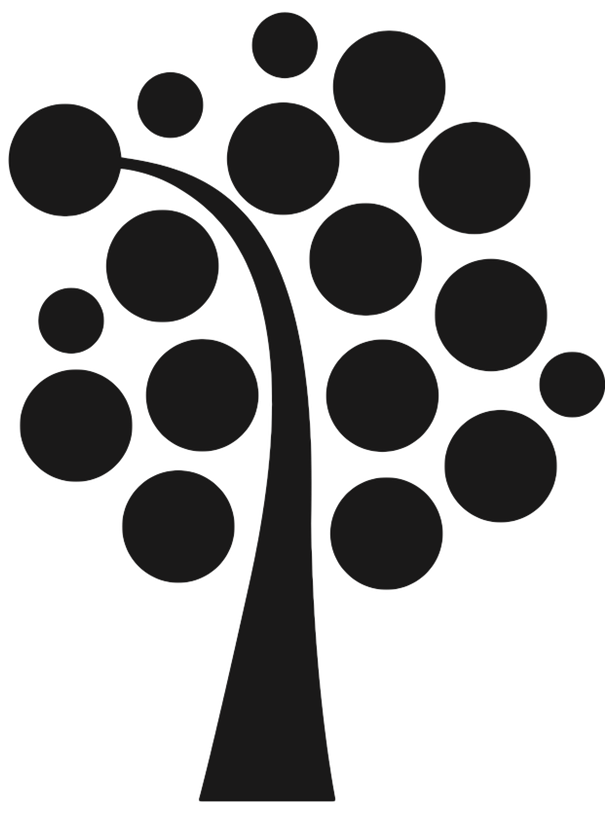
\includegraphics[keepaspectratio,scale=0.10]{figures/logo.png}
    }
}
\newcommand{
    \subsubsubsection}[1]{\paragraph{#1}\mbox{}\\
}
\title{	
\vspace{-8cm}
\begin{sidebar}
    \vspace{10cm}
    \normalfont\normalsize
    \Huge Bachelor Degree Project
    \vspace{-1.3cm}
\end{sidebar}
\vspace{3cm}
\begin{flushleft}
    \huge Applying Machine Learning to Reduce the Adaptation Space in Self-Adaptive Systems \\ 
    \it - an exploratory work \LARGE
\end{flushleft}
\null
\vfill
\begin{textblock}{6} (10,13)
\begin{flushright}
\begin{minipage}{\textwidth}
\begin{flushleft} \large
\author{}
\emph{Author:} Sarpreet Singh Buttar \\
\emph{Supervisors:} Dr. M.U. Iftikhar \\
\hspace{2.7cm}Prof. Danny Weyns\\
\emph{Semester:} Spring 2018 \\
\emph{Subject:} Computer Science \\
\end{flushleft}
\end{minipage}
\end{flushright}
\end{textblock}
}
\hyphenation{autonom-ously}
\begin{document}
\pagenumbering{gobble}
\newgeometry{left=5cm}
\AddToShipoutPicture*{\BackgroundPic}
\AddToShipoutPicture*{\BackgroundPicLogo}
\maketitle
\restoregeometry
\clearpage
\selectlanguage{english}
\begin{abstract}
\noindent 
Self-adaptive systems are capable of autonomously adjusting their behavior at runtime to accomplish particular adaptation goals. The most common way to realize self-adaption is using a feedback loop(s) which contains four actions: collect runtime data from the system and its environment, analyze the collected data, decide if an adaptation plan is required, and act according to the adaptation plan for achieving the adaptation goals. Existing approaches achieve the adaptation goals by using formal methods, and exhaustively verify all the available adaptation options, i.e., adaptation space. However, verifying the entire adaptation space is often not feasible since it requires time and resources. In this thesis, we present an approach that uses machine learning to reduce the adaptation space in self-adaptive systems. The approach integrates with the feedback loop and selects a subset of the adaptation options which are valid in the current situation. The approach is applied on the simulator of a self-adaptive Internet of Things application which is deployed in KU Leuven, Belgium. We compare our results with a formal model based self-adaptation approach called ActivFORMS. The results show that on average the adaptation space is reduced by 81.2\% and the adaptation time by 29.6 seconds compared to ActivFORMS results while achieving the same quality guarantees.

\vspace{.5cm}  
\noindent \textbf{Keywords:} Self-adaptive systems, Architecture-based self-adaptation, Adaptation space, MAPE-K feedback loop, DeltaIoT, ActivFORMS, Machine learning, Online supervised learning, Classification, Regression
\end{abstract}
\newpage
\noindent
\textbf {\large{Preface}}
\newline
\noindent
I would like to thank my supervisors, Dr. Muhammad Usman Iftikhar and Prof. Danny Weyns, for guiding me from the beginning to the end. Without their support, I would not be able to complete this thesis.
\newpage
\pagenumbering{gobble}
\tableofcontents
\newpage
\listoffigures
\newpage
\listoftables
\newpage
\lstlistoflistings
\newpage
\pagenumbering{arabic}
\section{Introduction}
Software is an essential part of modern society. It is highly used in various sectors such as telecommunication, automotive, electronics, robotics, etc. Software systems have to deal with complex issues while managing the activities of these sectors. One of the major issues is to handle uncertainties which appear at runtime, e.g., dynamic conditions of the environment in which the software systems operate, changing user goals, etc. These uncertainties are often unpredictable and may lead to undesired behavior in the software systems. To overcome this problem, software engineers have moved toward self-adaptation \cite{SEFSASARR-2009}, \cite{SEFSASASRR-2013}, \cite{SEFSASRCITPOA-2017}, \cite{SEOSASAOTAFC-2017}.


Self-Adaptation is a prominent approach that enables a software system to autonomously deal with the uncertainties at runtime in order to accomplish particular adaptation goals. Here, adaptation goals refer to a list of requirements which must be fulfilled by the software system. There are various types of adaptations such as architecture-based, self-healing, context-aware and mode-driven, etc. \cite{SEFSAS-2009}. In this thesis, we target the architecture-based adaptation \cite{TVOAC-2003} which decomposes the system into two parts: a managed system which needs adaptation and contains the domain logic, and a managing system which holds the adaptation logic. These systems communicate with each other through sensors and actuators. The managing system uses a feedback loop for achieving the adaptation goals of the managed system. A feedback loop is a control loop which provides a universal mechanism for self-adaptation. It contains four actions: collect, analyze, decide, and act. A common way to combine these actions is by using a MAPE-K feedback loop which was designed by IBM in 2003 \cite{AABFAC-2005} and is highly important in terms of its influence on self-adaptive and autonomic systems \cite{MAAMAPEKFLFSA-2015}. The MAPE-K feedback loop consists of five components named as monitor, analyzer, planner, executor, and knowledge, see figure \ref{SelfAdaptiveSystem}. 
\begin{figure}[H]
	\centering
	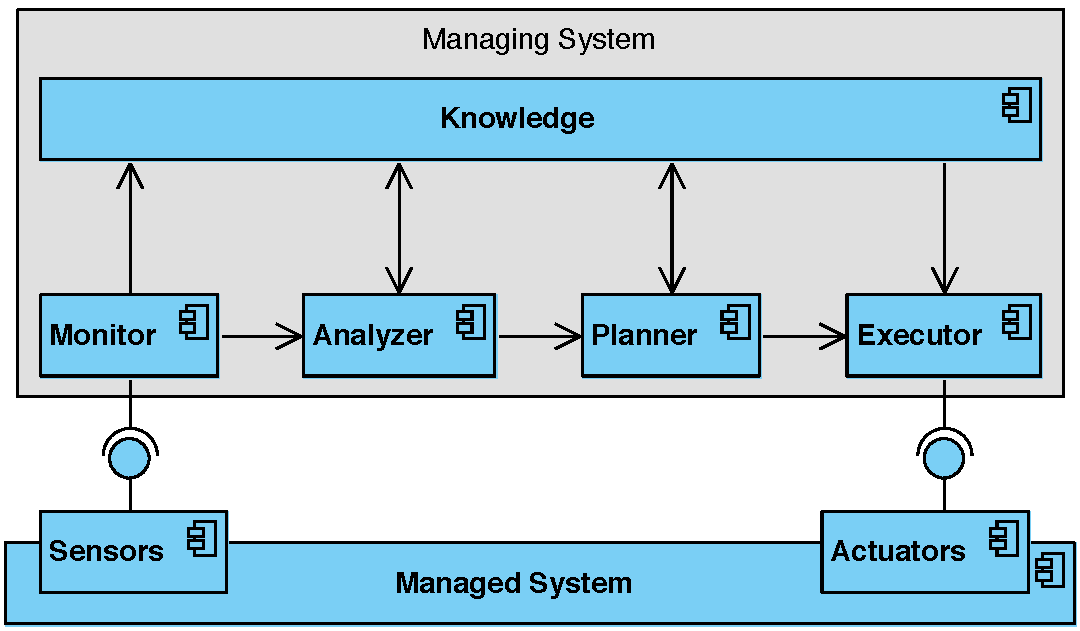
\includegraphics[keepaspectratio, width=\linewidth]{figures/SelfAdaptiveSystem.pdf}
	\caption{An overview of the architecture-based adaptation}
	\label{SelfAdaptiveSystem}
\end{figure}
The monitor collects runtime data from the managed system and its environment via sensors. Here, environment refers to an external entity in which the managed system operates. The analyzer analyzes the collected data to determine whether an adaptation is needed. If the adaptation is needed, the planner makes an adaptation plan. The executor adapts the managed system by executing the adaptation plan via actuators. The knowledge is a repository shared by MAPE (monitor, analyzer, planner, executor) components to maintain their data. For instance, the monitor saves the collected data, the planner saves the adaptation plan, etc. The MAPE components trigger one another after finishing their actions \cite{MBSARFSAS-2016}.

In this thesis, we consider self-adaptive systems where the managed system has a set of available adaptation options, i.e., adaptation space. Each adaptation option can affect the quality of the system. The managing system adapts the managed system by choosing one of the adaptation options which fulfill the adaptation goals.

Existing formal approaches in self-adaptive systems such as Active FORmal Models for Self-Adaptation (ActivFORMS) \cite{ACTIVFORMS-2014}, \cite{TRSMCFSAS-2016} and Runtime Quantitative Verification (RQV) \cite{SASNQVAR-2012}, \cite{ETSASWDAC-2017} use model checking techniques to achieve the adaptation goals at runtime. These approaches connect the analyzer with a model checker which verifies the violations of the adaptation goals with all the available adaptation options. This runtime verification requires time and resources, e.g., CPU usage and memory, because the adaptation space may consist of hundreds or even thousands of adaptation options \cite{TLFIMPIHCS-2017}, \cite{DQMAOISBS-2011}. Therefore, these approaches are limited to small scale applications.

In this thesis, we aim to investigate how to reduce the adaptation space to a subset of the adaptation options which are valid in the current situation of the system. This subset will be further verified by the feedback loop which will select the best adaptation option. By reducing the adaptation space, we are aiming to lower the adaptation time, i.e., the time feedback loop takes to adapt the system, while having the same quality guarantees provided by the model checking approaches. Concretely, we focus on using machine learning for this purpose which can be integrated with a model checking approach and can learn on the fly which adaptation options should be selected. We apply our approach on a self-adaptive Internet of Things (IoT) application and compare the results with ActivFORMS.
\subsection{Background}
In this section, we briefly introduce the theories which are related to this thesis. We start by explaining the fundamentals of machine learning. After that, we describe the self-adaptive IoT application called DeltaIoT on which we applied our suggested approach. In the end, we illustrate ActivFORMS approach.
\subsubsection{Machine Learning}
In general machine learning is when learning algorithms make predictions by using experience obtained in the past. Typically the experience consists of collected data, such as a set of labeled examples, where the quality and the number of examples are essential. The idea is that the more high quality examples are presented to the learning algorithms, the more accurate their predictions can become. Machine learning consists of various learning scenarios such as supervised learning, unsupervised learning, semi-supervised learning, reinforcement learning, etc., \cite{FOML-2012}. In this thesis, we focused on supervised learning which involves two sequential phases. First, the training phase in which the learning algorithm learns from a set of labeled examples known as a training dataset. Second, the testing phase in which the learning algorithm receives a testing dataset and predicts its output \cite{ML-2016}, see table \ref{ExampleDatasets}.
\begin{table}[H]
	\begin{subtable}{.5\linewidth}
		\centering
		\begin{tabular}{c|c|c|c}
			\hline
			\multicolumn{1}{c|}{} & \multicolumn{2}{c|}{\textbf{Features}} & \multicolumn{1}{c}{\textbf{Target}} \\
			\cline{1-3} \cline{3-4}
			Item & Height(cm) & Weight(kg) & Age \\
			\hline
			1 & 180 & 75.9 & 34 \\
			\hline
			2 & 160 & 60 &  16 \\
			\hline
			3 & 170 & 85 & 40 \\
			\hline
		\end{tabular}
		\caption{Training dataset}
	\end{subtable}
	\begin{subtable}{.5\linewidth}
		\centering
		\begin{tabular}{c|cc}
			\hline
			\multicolumn{1}{c|}{} & \multicolumn{2}{c}{\textbf{Features}} \\
			\cline{1-3}
			Item & Height(cm) & Weight(kg) \\
			\hline
			1 & 150 & 65.9 \\
			\hline
			2 & 140 & 50 \\
			\hline
			3 & 184 & 90 \\
			\hline
		\end{tabular}
		\caption{Testing dataset}
	\end{subtable} 
	\caption{Example of the training and testing datasets}
	\label{ExampleDatasets}
\end{table}
A training dataset contains one or more items. Each item has attributes known as features and an output known as a target. A testing dataset contains only the features and no items from the training dataset. The training and testing datasets must contain numeric values in order for the learning algorithm to work \cite{HOMLWSLATF-2017}.

Classification, regression, ranking, etc., are common approaches used in supervised learning. In this thesis, we focused on the classification and regression. In classification, the targets in the training dataset are classes, whereas in regression they are real values, see table \ref{DatatsetsForApproaches}.
\begin{table}[H]
	\begin{subtable}{.5\linewidth}
		\centering
		\scalebox{0.9}{
			\begin{tabular}{c|c|c|c}
				\hline
				\multicolumn{1}{c|}{} & \multicolumn{2}{c}{\textbf{Features}} & \multicolumn{1}{|c}{\textbf{Target}} \\
				\cline{1-1} \cline{2-3} \cline{4-4}
				Item & Height(cm) & Weight(kg) & Age \\
				\hline
				1 & 180 & 75.9 & 1 \\
				\hline
				2 & 160 & 60 &  0 \\
				\hline
				3 & 170 & 85 & 1 \\
				\hline
			\end{tabular}
		}
		\caption{Classification}
		\label{Classification}
	\end{subtable}
	\begin{subtable}{.5\linewidth}
		\centering
		\scalebox{0.9}{
			\begin{tabular}{c|c|c|c}
				\hline
				\multicolumn{1}{c|}{} & \multicolumn{2}{c}{\textbf{Features}} & \multicolumn{1}{|c}{\textbf{Target}} \\
				\cline{1-1} \cline{2-3} \cline{4-4}
				Item & Height(cm) & Weight(kg) & Age \\
				\hline
				1 & 180 & 75.9 & 34 \\
				\hline
				2 & 160 & 60 &  16 \\
				\hline
				3 & 170 & 85 & 40 \\
				\hline
			\end{tabular}
		}
		\caption{Regression}
		\label{Regression}
	\end{subtable} 
	\caption{Example of the training datasets used in classification and regression}
	\label{DatatsetsForApproaches}
\end{table}
Table \ref{Classification} shows that the targets are represented by class 1 and 0. The items with class 1 have age >=18, whereas the remaining item has age <18. In contrast, the targets in table \ref{Regression} are real values. Therefore, in classification, the learning algorithm is trained to predict the classes of the items, and in regression, it is trained to predict the real values of the items.

Supervised learning can be done either during design time (offline learning) or runtime (online learning). In this thesis, we used online learning. In online learning, the training and testing phases are intermixed which enables the learning algorithm to interact with them multiple times. For instance, the learning algorithm is in the testing phase and predicts the targets of the items. Then it moves in the training phase and receives the same items with their actual targets. These interactions enable the learning algorithm to continuously adapt itself according to the constant flow of data. Therefore, online learning fits in various application scenarios such as learning in an uncertain environment, lifelong learning, etc. These scenarios are often present whenever a system behaves autonomously such as auto driving or robotics. Furthermore, there are some interactive scenarios where online learning becomes mandatory, e.g., the training dataset is dependent on human feedback over time \cite{ILAAA-2016}.
\subsubsection{DeltaIoT: Internet of Things Application}
DeltaIoT is an architecture-based self-adaptive IoT application which autonomously manages the settings of IoT device (motes) under uncertain operating conditions in order to maintain the quality requirements \cite{DELTAIOT-2017}. Examples of uncertain operating conditions are dynamic traffic of the motes, communication interference between the motes, etc. It is constructed as a smart mesh network with 15 motes. These motes are connected via a wireless link and equipped with three different types of sensors: RFID, passive infrared, and heat sensors. DeltaIoT is deployed at the Computer Science Department of KU Leuven, Belgium, see figure \ref{DeltaIoT}.
\begin{figure}[H]
	\centering
	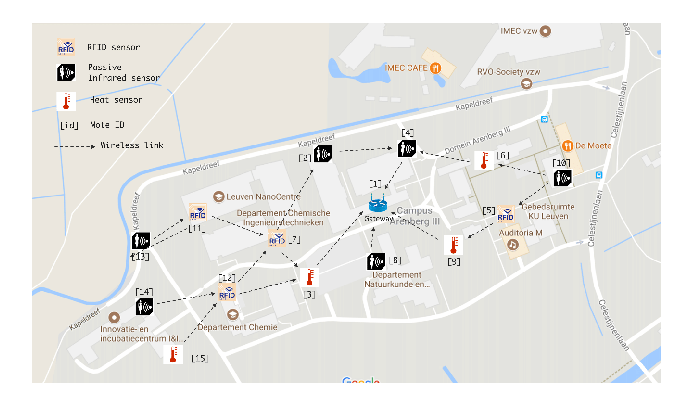
\includegraphics[keepaspectratio, width=\linewidth]{figures/DeltaIoT.pdf}
	\caption{DeltaIoT at KU Leuven}
	\label{DeltaIoT}
\end{figure}
The RFID sensors provide access control to the labs. The passive infrared sensors monitor the occupancy status of the building. The heat sensors record the temperature. These sensors deliver their sensor data to the IoT gateway which is placed at the central monitoring facility. Communication in the smart mesh network relies on time synchronization. The communication is formulated in cycles where each cycle contains a fixed amount of communication slots. A communication slot allows two motes (sender and receiver) to communicate with each other. The communication slots are adequately divided between the motes.

DeltaIoT has many quality requirements such as the average packet loss should be under 10\%, the energy consumption of the motes should be minimum, the latency should be under 5\%. etc. There are two primary uncertainties which have a high impact on the quality requirements. First, external interference in the network, e.g., weather conditions, other WiFi signals, etc., affects the quality of communication and as a result, the packet loss may increase. Second, fluctuation in the traffic load of the motes may vary from time to time, e.g., a passive infrared sensor only produces the packets when a human motion is detected. However, during working hours, the traffic load can increase which may also increase the packet loss.

The quality requirements of DeltaIoT are decided by two factors:
\begin{enumerate}
	\item The power settings of the motes.
	\item The distribution of the packets.
\end{enumerate}
The power settings of each mote can be from 0 to 15. For increasing the lifetime of the motes, it must be configured optimally. For instance, the high power settings increase the energy consumption of the motes, and low power settings reduce the signal strength of the motes which leads to a high packet loss. Similarly, a mote with two parents can distribute the packets by sending 0\% to one parent and 100\% to the other, 20/80, ...., 100/0, etc. There are three motes (mote 7, 10, and 12) in the network which have two parents, see figure \ref{DeltaIoT}. 

In this thesis, we consider the following quality requirements for DeltaIoT:
\begin{enumerate}
	\item The average packet loss should be under 10\%.
	\item The energy consumption of the motes should be minimum. 
\end{enumerate}
DeltaIoT provides a simulator for the offline experimentation. In this thesis, we used this simulator for conducting the experiments. The simulator allows to adjust the distribution of the packets and power settings. The simulator also allows to manage uncertainties in the environment of DeltaIoT. This can be done by configuring the traffic load and signal to noise ratio (SNR) which represents the noise in the environment due to external interference. If the interference is high, the SNR goes down which leads to higher packet loss. Since DeltaIoT realizes architecture-based adaptation its quality requirements become its adaptation goals.
\subsubsection{ActivFORMS} \label{Activforms}
ActivFORMS (Active FORmal Models for Self-Adaptation) is a model based approach that provides guarantees to achieve the adaptation goals of self-adaptive systems at runtime %\cite{AMBATESASWG-2017}
. Figure \ref{ActivFORMSOverview} provides an overview of ActivFORMS. 
\begin{figure}[H]
	\centering
	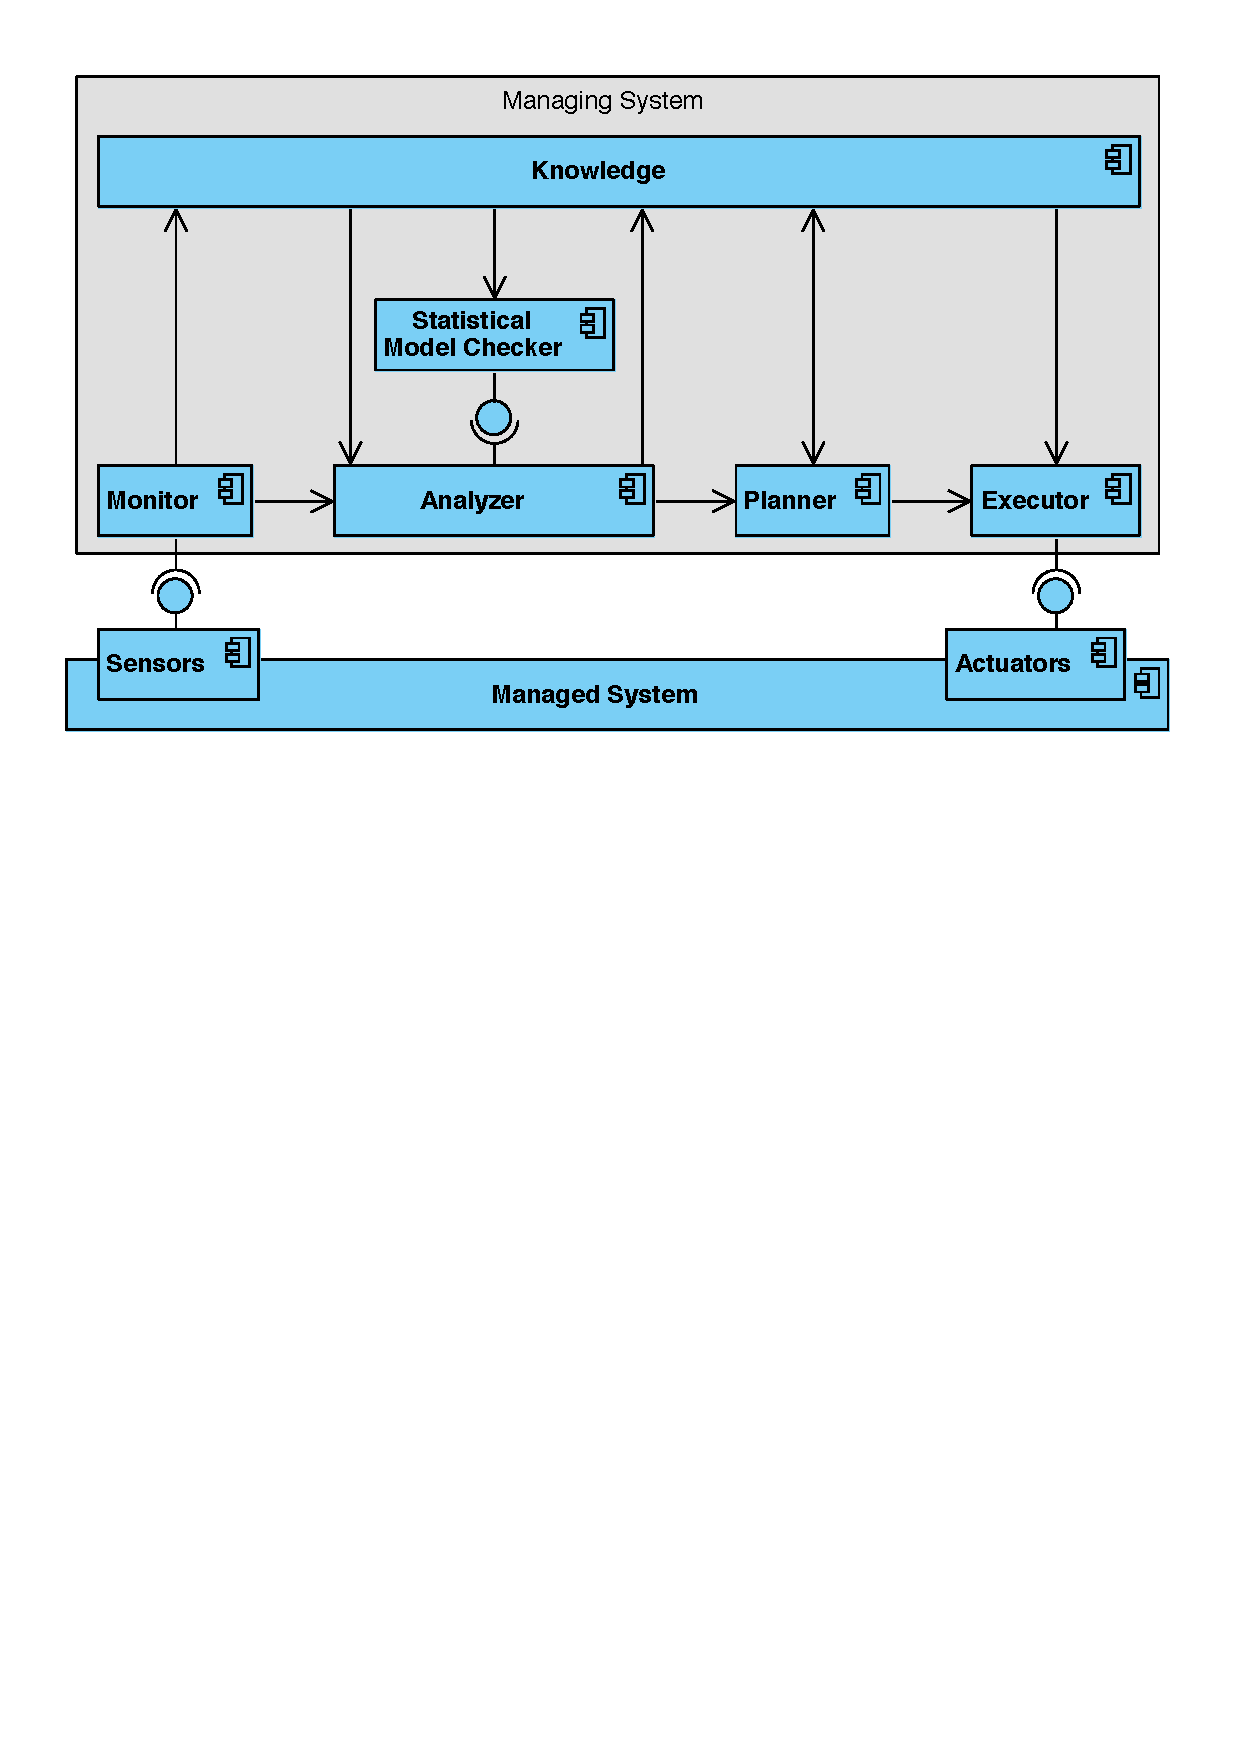
\includegraphics[keepaspectratio, width=\linewidth]{figures/ActivFORMSOverview.pdf}
	\caption{An overview of ActivFORMS}
	\label{ActivFORMSOverview}
\end{figure}
ActivFORMS extends the MAPE-K loop with a statistical model checker that connects with the analyzer. The statistical model checker provides support to the analyzer to estimate the quality requirement for each adaptation option. The statistical model checker uses simulation and statistical techniques to estimate the quality requirements. The accuracy of the estimated values is dependent on the number of simulations. The high accuracy requires more simulations which takes more time and resources such as CPU usage and memory. Figure \ref{ActivFORMSRuntimeView} shows the runtime components of ActivFORMS. 
\begin{figure}[H]
	\centering
	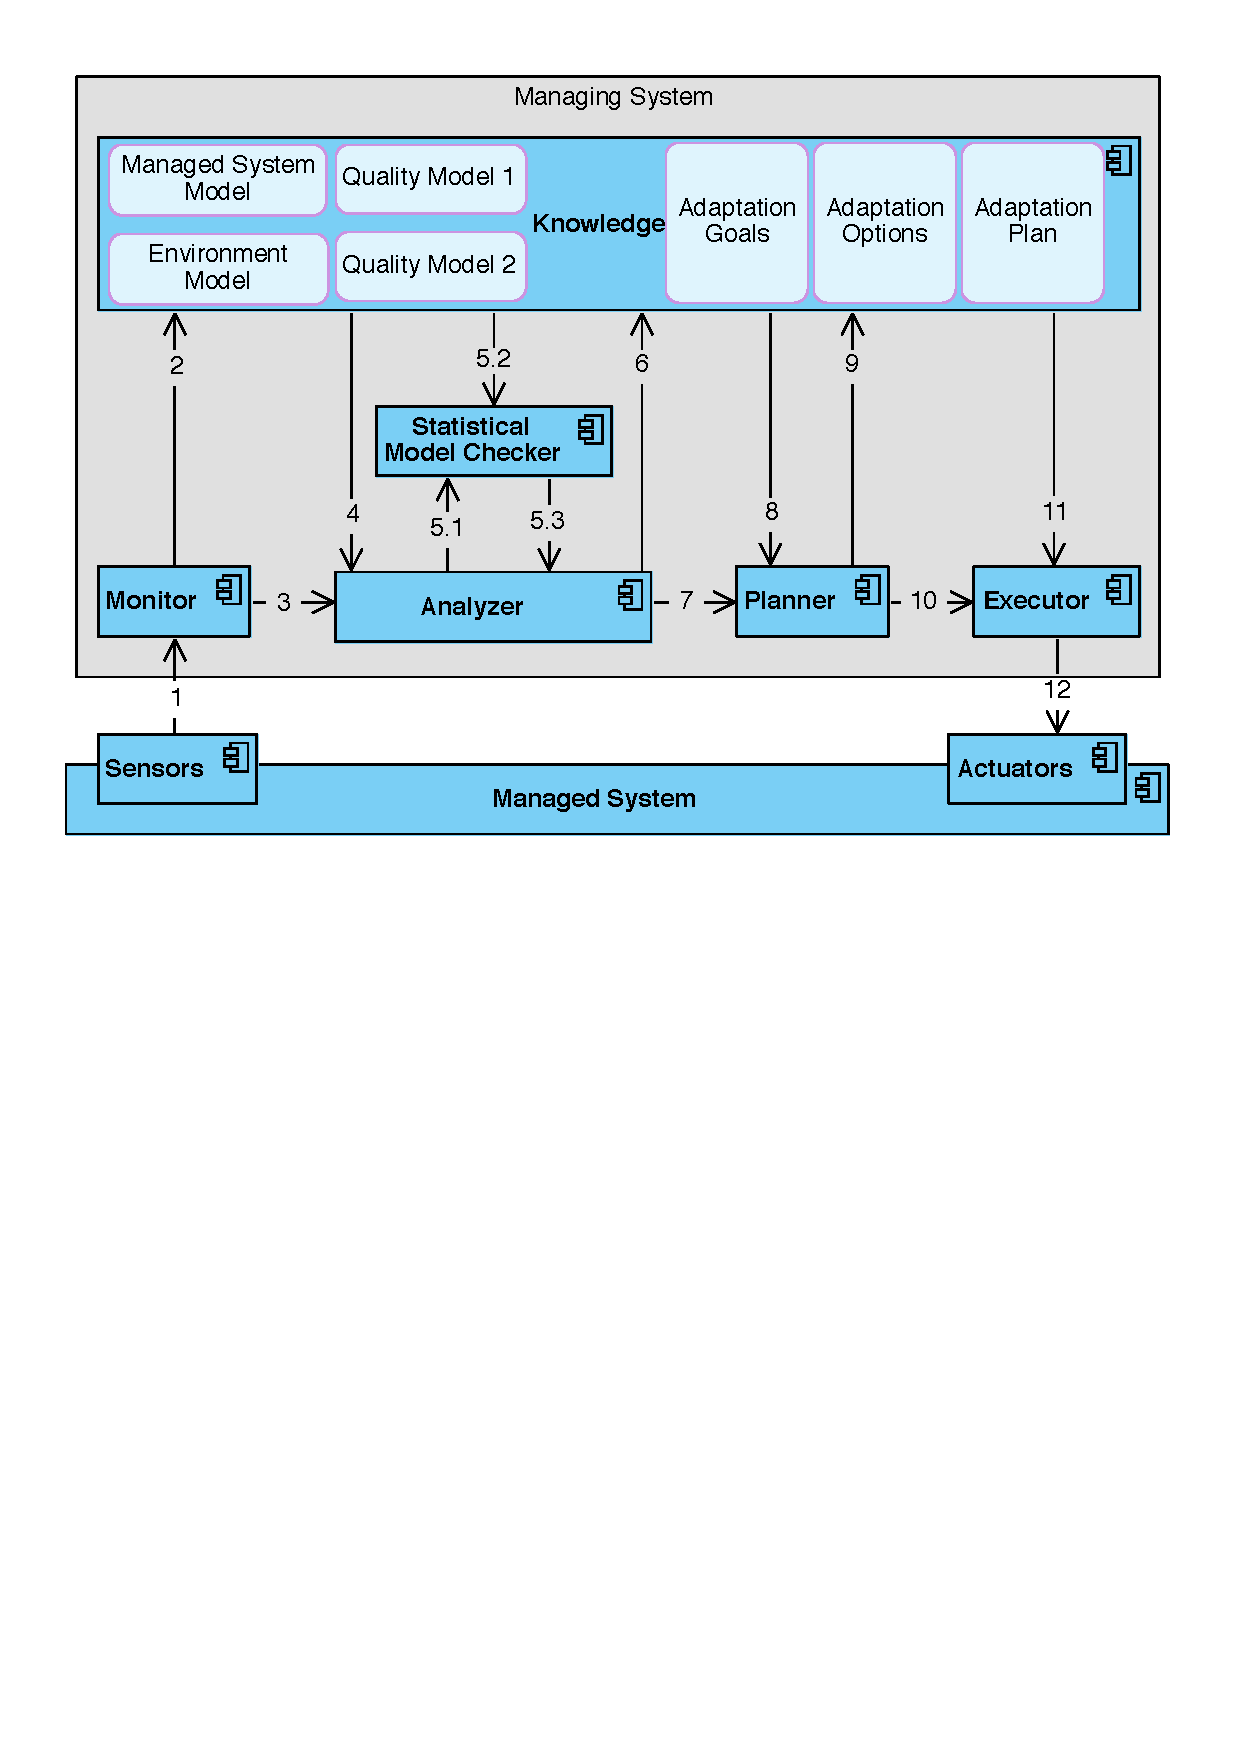
\includegraphics[keepaspectratio, width=\linewidth]{figures/ActivFORMSRuntimeView.pdf}
	\caption{A runtime view of ActivFORMS}
	\label{ActivFORMSRuntimeView}
\end{figure} 
The knowledge repository contains many elements such as managed system model, environment model, quality models, adaptation goals, adaptation options and adaptation plan. The managed system model holds the current uncertain values of the managed system. Similarly, the environment model holds the current uncertain values of the environment in which the managed system operates. Each quality model represents the managed system and its environment for the quality requirement which is subject to adaptation. The managed system, environment, and quality models are called runtime models. These models are parametrized which enable them to capture the values of different uncertainties at runtime. The adaptation goals are a set of requirements which are followed to select the best adaptation option. The adaptation options represent a set of different configurations. Each adaptation option has a placeholder where it holds the value of each quality requirement (estimated by the statistical model checker) which is subject to adaptation. The adaptation plan consists of adaptation actions which are required to adapt the managed system to accomplish the adaptation goals. Here we present the flow of ActivFORMS.
\begin{enumerate}
	\item The monitor collects runtime data from the managed system and its environment. The collected data contains the current uncertain values of the managed system and its environment.
	\item The monitor updates the runtime models with the collected data.
	\item The monitor triggers the analyzer.
	\item The analyzer reads the adaptation options, managed system and environment models. 
	\item First, the analyzer feeds the statistical model checker with the adaptation options and current uncertain values of the managed system and environment. Second, for each adaptation option, the statistical model checker simulate each quality model and estimate the quality values. Third, the statistical model checker sends the estimated values back to the analyzer.
	\item The analyzer updates the placeholder of the adaptation options with the corresponding estimated values and determines if an adaptation is needed.
	\item If the adaptation is needed, the analyzer triggers the planner.
	\item The planner reads the adaptation options and goals. The planner ranks the adaptation options according to the adaptation goals and makes an adaptation plan for the top ranked adaptation option.
	\item The planner saves the adaptation plan.
	\item The planner triggers the executor.
	\item The executor reads the adaptation plan.
	\item The executor adapts the managed system by executing the adaptation plan via actuators.
\end{enumerate}
\subsection{Problem Formulation}
Existing formal approaches such as ActivFORMS and RQV use model checking to achieve the adaptation goals of self-adaptive systems. These approaches use exhaustive verification to verify all the adaptation options which enable them to find the best adaptation option. However, model checking at runtime requires time and resources such as CPU power and memory. The time and resources are directly dependent on the size of the adaptation space. This can be overhead for some self-adaptive systems which need fast adaptation. Hence, we aim to use machine learning to reduce the adaptation space to only the relevant adaptation options. This will enable the formal approaches to achieve the adaptation goals by only analyzing the relevant adaptation options. The reduced adaptation space will also save time and resources.
\subsection{Motivation}
A recent research applied ActivFORMS on DeltaIoT to achieve its quality requirements 
%\cite{AMBATESASWG-2017}. 
It shows that often there are few adaptation options that are able to achieve the quality requirements, see figure \ref{DeltaIoT-ActivFORMS}. 
\begin{figure}[H]
	\centering
	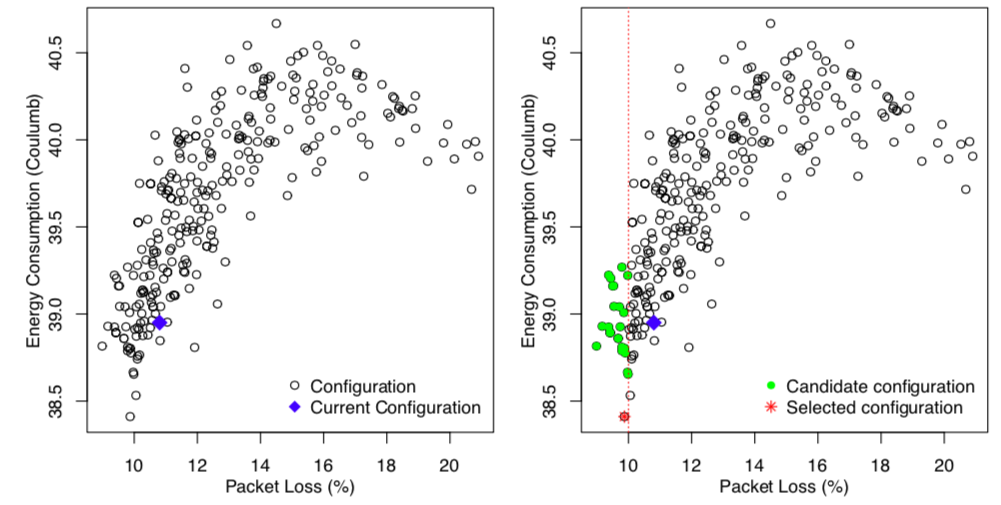
\includegraphics[keepaspectratio, width=\linewidth]{graphs/DeltaIoT-ActivFORMS.png}
	\caption{Selection of the best adaptation option with ActivFORMS %\cite{AMBATESASWG-2017}
	}
	\label{DeltaIoT-ActivFORMS}
\end{figure}
The left hand side graph shows all the available adaptation options for DeltaIoT. ActivFORMS used statistical model checker to estimate the quality requirements of each adaptation option. The current adaptation option during the analysis is represented by a diamond dot. On the right hand side, the green filled dots represent those adaptation options which fulfill the packet loss quality requirement. The red asterisk dot represents the best adaptation option selected by the planner because it has minimum energy consumption compared to others.

It is clear from the above figure that there is no need to verify the entire adaptation space. Rather, it is possible to achieve the quality requirements by selecting a subset of the adaptation options. This will not only reduce the adaptation space but also drop the adaptation time.
\subsection{Research Question}
\begin{table}[H]
	\centering
	\begin{tabular}{|p{1cm}|p{11cm}|}
		\hline
		\textbf{RQ1} & How to reduce the adaptation space in self-adaptive systems using machine learning? \\
		\hline
	\end{tabular}
	\caption{Research Question}
\end{table}
With this research question, we aim to achieve a reduction in the adaptation space so only relevant adaptation options could be chosen by the MAPE-K feedback loop. The reduction in the adaptation space should be done in a way that the quality requirements of the self-adaptive system are still achievable. This will reduce the adaptation time and inherently allows the MAPE-K feedback loop to deal with large adaptation spaces.
\subsection{Scope/Limitation}
We divide the scope of this thesis into four categories.
\begin{enumerate}
	\item In machine learning we only focused on online supervised learning with classification and regression approaches.
	\item For evaluation, we limit to only the DeltaIoT application.
	\item The machine learning is applied to only one quality requirement, i.e., packet loss. For energy consumption, we use model checking.
	\item We consider that adaptation options are fixed and do not change at runtime.
\end{enumerate}
\subsection{Target Group}
With our approach, we aim to target both industry and academia readers. For instance, DeltaIoT which is used for the evaluation in this thesis is deployed in KU Leuven, Belgium by a company called VersaSense. It could be useful for such systems to explore our approach. In academia, it will be useful for model checking approaches that use exhaustive verification to speed up their adaptation.
\subsection{Outline}
This thesis is organized as follows. In section \ref{Method}, we explain the scientific methods. Then in section \ref{Approach}, we present our approach. Furthermore, in section \ref{Implementation}, we apply of our approach on DeltaIoT. We discuss the results in section \ref{ResultsAndAnalysis}. In section \ref{RealtedWork}, we present the work related to our approach. Finally, we conclude this thesis and provide directions for future work in section \ref{Conclusion}. 
\newpage
\section{Method} \label{Method}
To answer the research question we used the controlled experiment method. This method requires two variables: an independent variable(s) which represents the input, and a dependent variable(s) which is affected by the input. The dependent variable(s) is also known as result. We used the controlled experiment method to measure the quantitative data of DeltaIoT with and without machine learning approaches. 
\subsection{Method Description}
For machine learning, we used two different approaches, i.e., classification and regression, and we used a statistical model checker to verify the reduced adaptation space. For without machine learning we used ActivFORMS approach that uses a statistical model checker to explore the adaptation space as explained in the section \ref{Activforms}. 

We performed two controlled experiments. In the first experiment, an independent variable is an approach (ActivFORMS, classification or regression). The dependent variables are the adaptation time, adaptation space, packet loss, and energy consumption. The goal of this experiment is to compare the approaches based on the values of the dependent variables. In the second experiment, an independent variable is an approach (ActivFORMS, classification or regression). The dependent variable is the adaptation space. The goal of this experiment is to investigate whether the adaptation options selected by classification and regression are similar to ActivFORMS.
\subsection{Reliability and Validity}
For reliability, we uploaded the implementation of our approach and the quantitative data from the experiments on GithHub, see appendix \ref{Appendix}. This allows any interested reader to replicate our work.

We evaluated our approach only on the simulator provided by DeltaIoT. This can lead to an external validity threat because we did not use the real system. However, this is not considered a big threat to the validity of our work, as the simulator is a replica of the real system and therefore should generate the same results.
\newpage
\section{Approach} \label{Approach}
In this section, we present our approach that uses machine learning to reduce the adaptation space in self-adaptive systems. We start with an overview of our approach. Then we explain how online supervised learning is used in our approach. In the end, we explain how our approach will work in all the phases of online supervised learning.
\subsection{Overview}
Our approach follows the principle of the architecture-based self-adaptation. Recall that the architecture-based self-adaptation decomposes the system into a managed system which needs adaptation and contains the domain logic, and a managing system which holds the adaptation logic. Our approach embeds machine learning and the model checker in the managing system so that they can integrate with the MAPE-K feedback loop. Figure \ref{ArchitectureOverview} shows the architecture of our approach.
\begin{figure}[H]
	\centering
	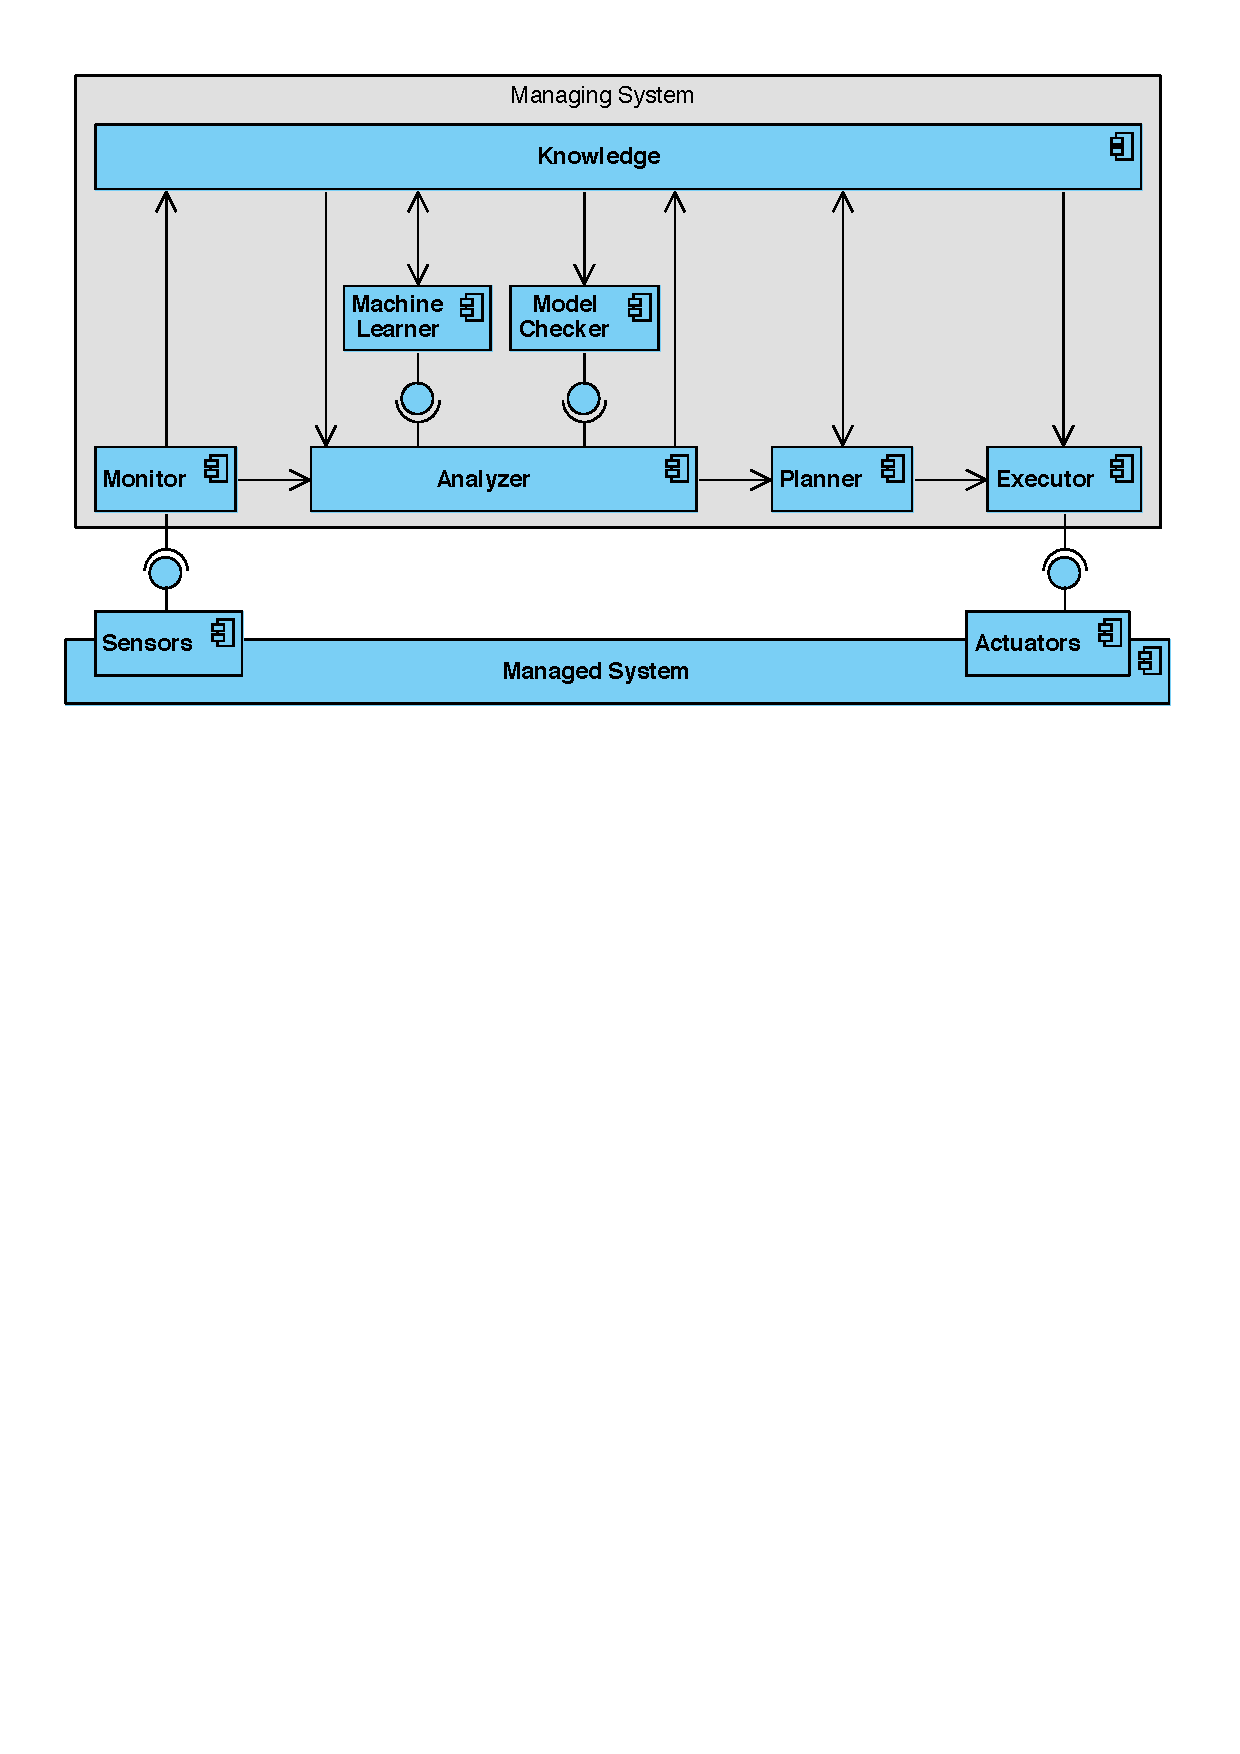
\includegraphics[keepaspectratio, width=\linewidth]{figures/ArchitectureView.pdf}
	\caption{Architecture of our approach}
	\label{ArchitectureOverview}
\end{figure}
The analyzer connects with the machine learner and the model checker. The machine learner supports the analyzer by selecting a subset of the adaptation options which are valid in the current situation. Whereas, the model checker verifies the selected adaptation options and provide the estimate of the quality requirements. Our approach is not limited to any particular type of machine learning. Any type, e.g., supervised learning, unsupervised learning, reinforcement learning, etc., with online learning can be used. Similarly, our approach is not limited to a particular model checker. Any type of model checker (statistical or probabilistic) can be used.

Recall that the monitor collects runtime data from the managed system and its environment via sensors and updates the runtime models with the collected data. Then the analyzer reads the adaptation options, managed system, and environment models. Here, we connect the analyzer with the machine learner which predicts the values of the quality requirements for each adaptation option. The analyzer then uses the predicted values to select the adaptation options which are relevant under the current uncertainties. The relevant adaptation options are then further verified by the model checker. After that, the analyzer uses the verified results of the relevant adaptation options to update the machine learner. This enables the machine learner to adapt itself according to the verified results and makes more accurate predictions in the future. Recall that in online learning, the learning algorithm predicts the targets of the items, and then also receives the actual targets. Therefore, our approach requires a model checker which can compute the actual targets (the values of the quality requirements) at runtime. Then the analyzer invokes the planner which reads the verified adaptation options, finds the best adaptation option, and makes an adaptation plan. In the end, the executor adapts the managed system by executing the adaptation plan via actuators.

Recall that there machine learning consists of various learning scenarios. In this thesis, we focused only on online supervised learning. Here we explain how it can be used in our approach.
\subsection{Online Supervised Learning}
In online supervised learning, there are training and testing phases which intermix with each other. In training phase, we train the learning algorithms whereas, in testing, the learning algorithms make predictions. However, to start with online supervise learning we need to go through with the general phase of machine learning called preprocessing. Figure \ref{OnlineSupervisedLearning} shows an overview of these phases. We start explaining the preprocessing and then we discuss how the training and testing phases are used in our approach.
\begin{figure}[H]
	\centering
	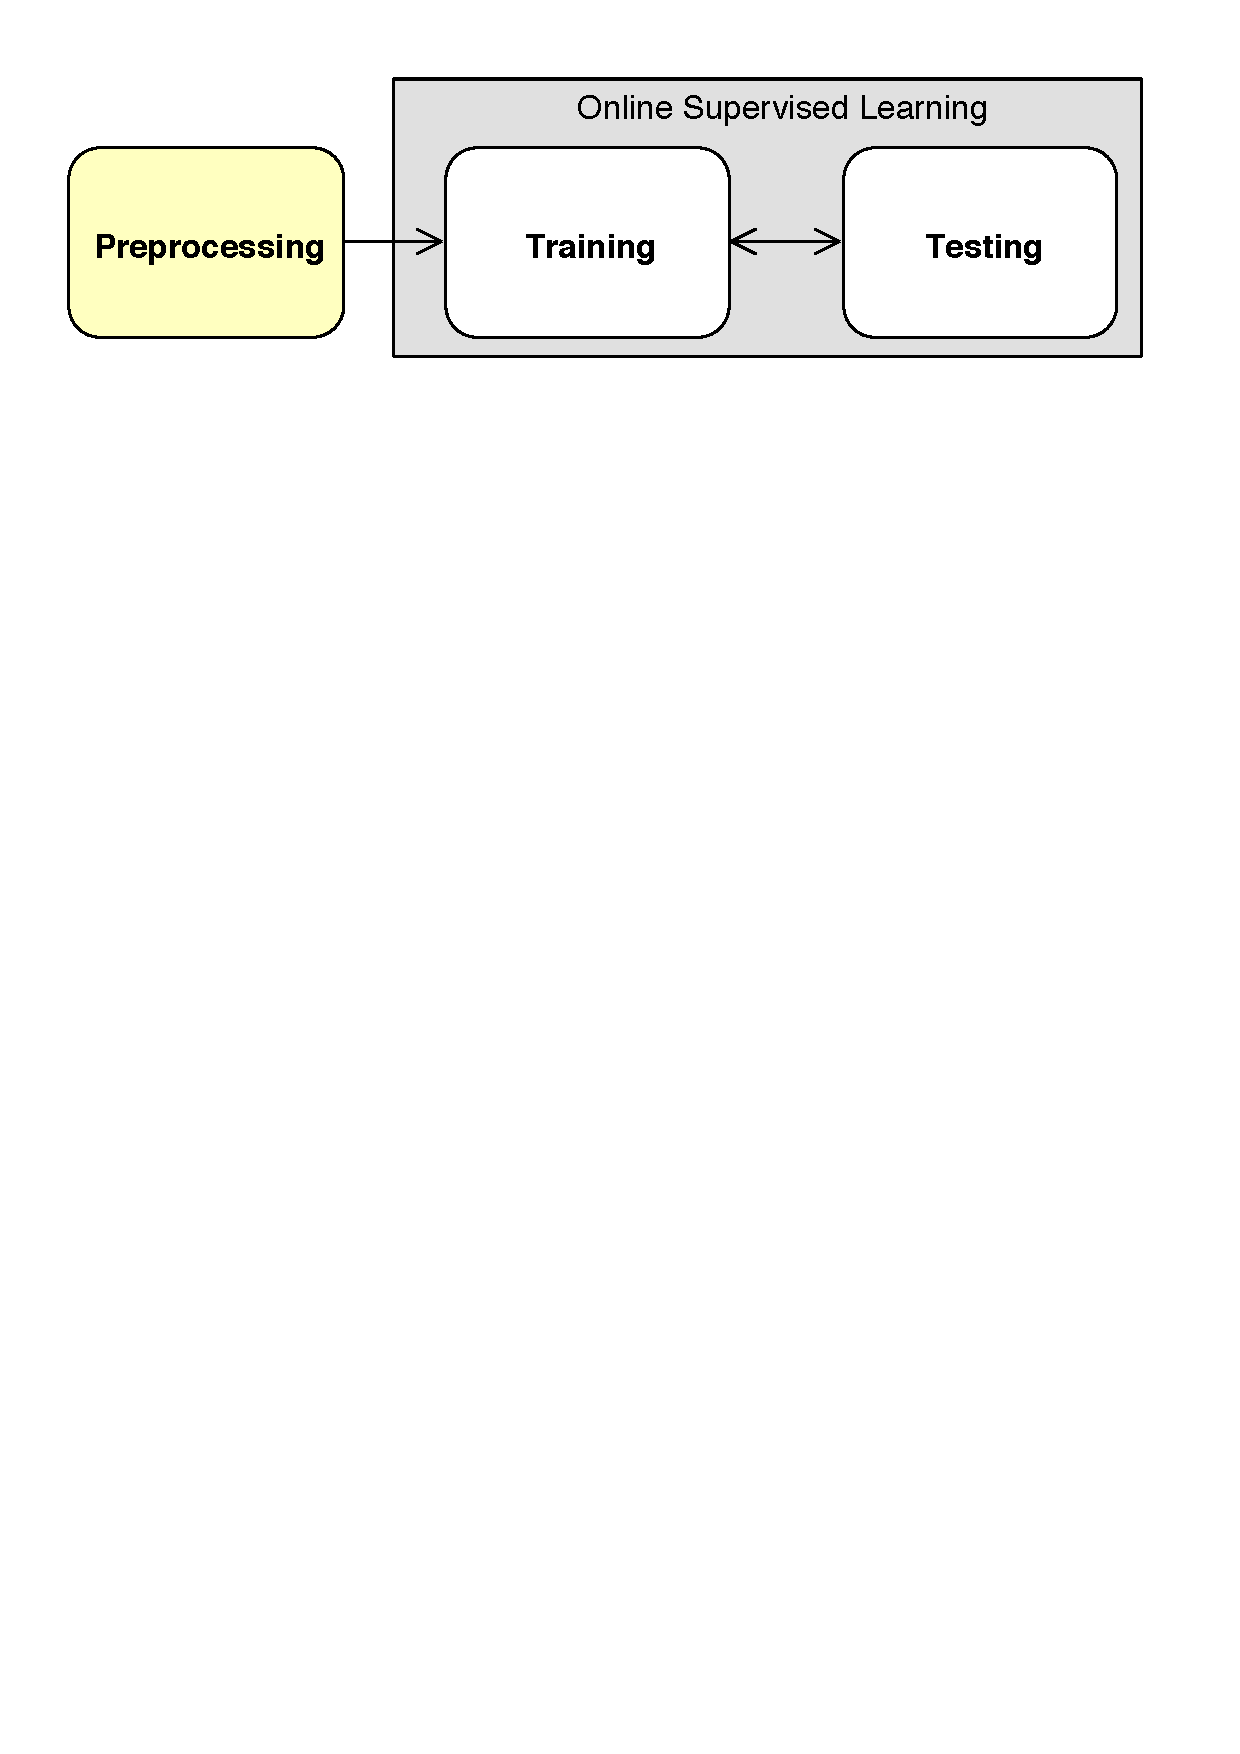
\includegraphics[keepaspectratio, width=\linewidth]{figures/OnlineSupervisedLearning.pdf}
	\caption{An overview of online supervised learning}
	\label{OnlineSupervisedLearning}
\end{figure}
\subsubsection{Preprocessing} 
Preprocessing plays an important role in reducing redundancy in the data, increasing the accuracy of the learning algorithms, and reducing the training time of the learning algorithms \cite{HOMLWSLATF-2017}, \cite{SLMLIP-2011}, \cite{LSLMLIP-2013}. It includes various processes such as data preprocessing, feature extraction, feature scaling, etc. The usage of these processes depends on various factors such as the machine learning type (supervised learning, unsupervised learning, etc.) and the approach (classification, ranking, etc.) used in the machine learning type. We selected some of the processes which are relevant to the online supervised learning with classification and regression approaches. The selected processes are data preprocessing, feature selection, feature scaling, and model selection. Figure \ref{Preprocessing} shows how the selected processes can be used in self-adaptive systems.
\begin{figure}[H]
	\centering
	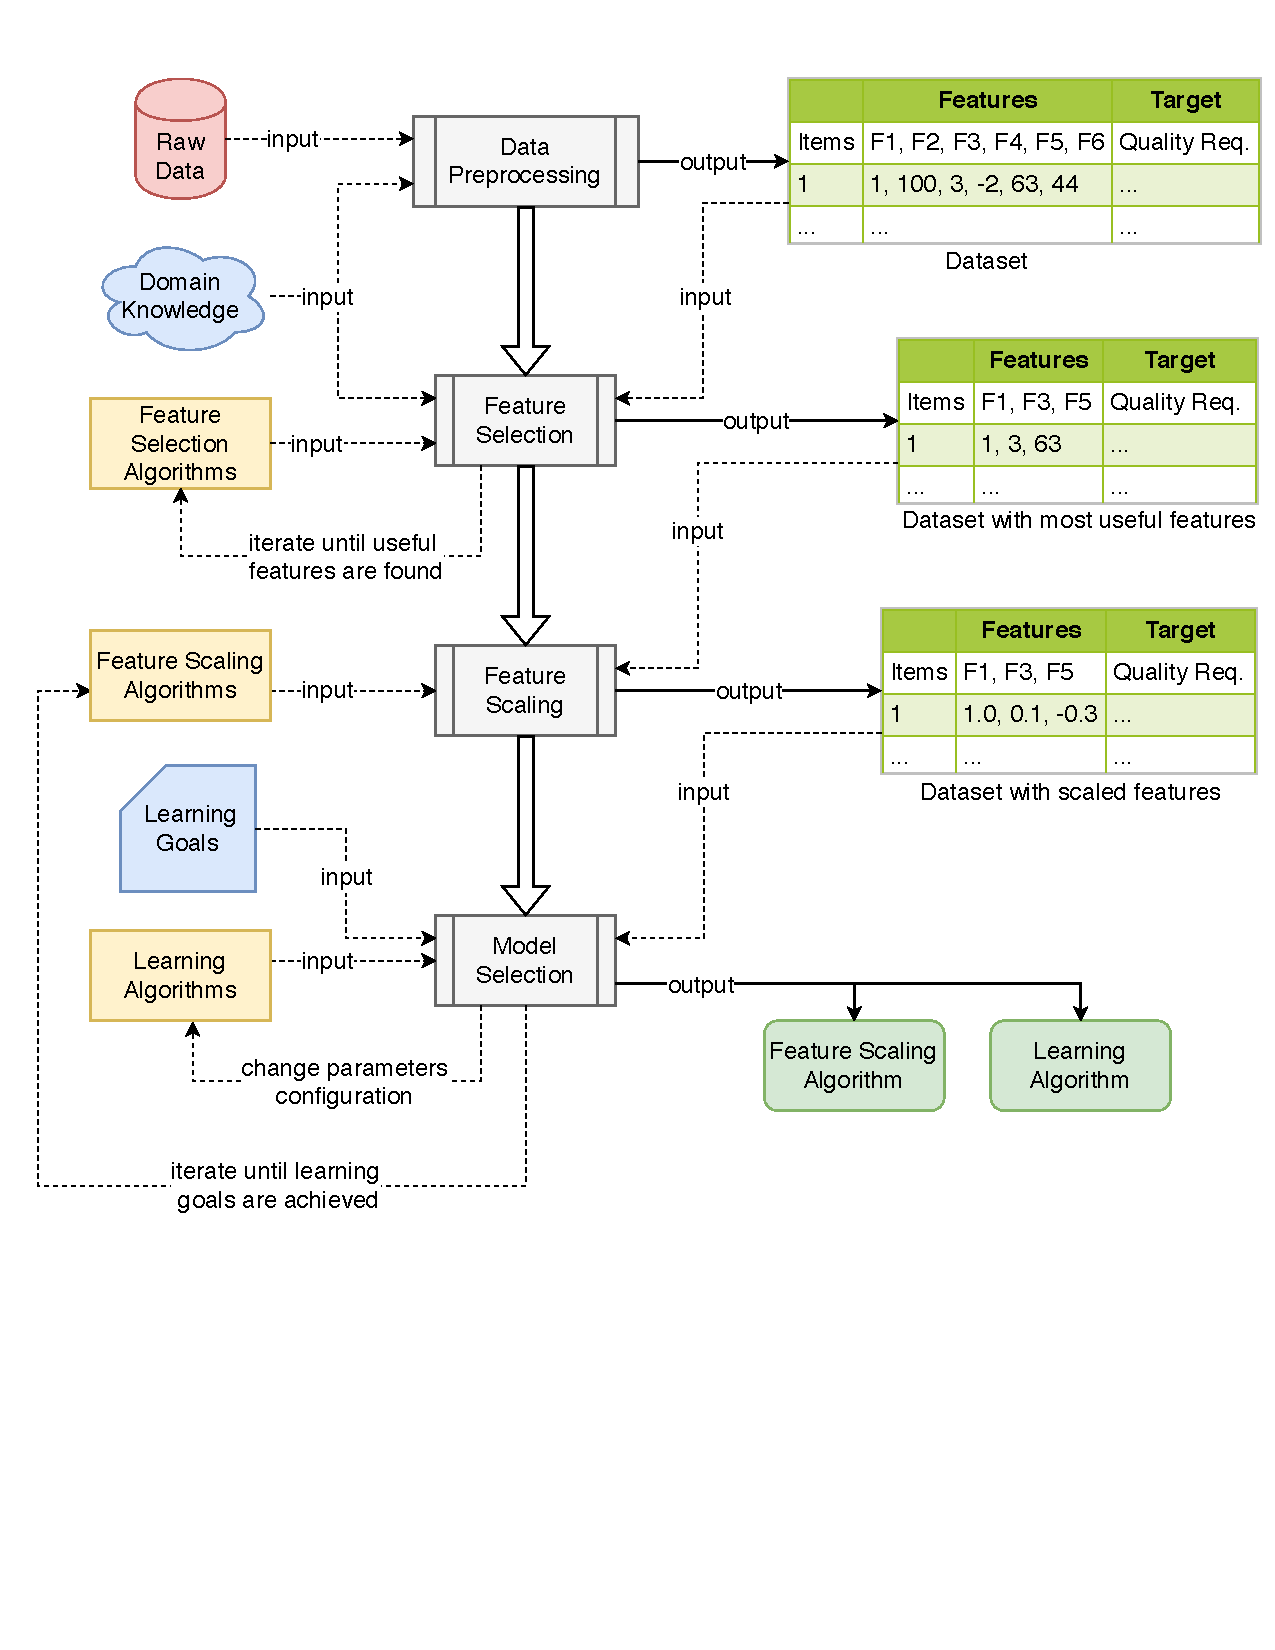
\includegraphics[keepaspectratio, width=\linewidth]{figures/Preprocessing.pdf}
	\caption{Preprocessing in self-adaptive systems}
	\label{Preprocessing}
\end{figure}
\subsubsubsection{Data Preprocessing}
Data preprocessing is used to prepare the raw data for the learning algorithms \cite{HOMLWSLATF-2017}. We suggest to collect raw data which contains examples of the adaptation decisions made by the MAPE components. For instance, when the uncertain values of the managed system and its environment are $\alpha$, the value of the quality requirement is $\gamma$ with an adaptation option whose configurations value are $\beta$. Such examples can be collected from the knowledge repository once the analyzer updates the adaptation options. The uncertain values can be achieved from the runtime models which also lie in the knowledge repository. We suggest to collect a reasonable amount of such examples such as 10k in order to get good results from the preprocessing processes. The $\alpha$, $\beta$ and $\gamma$ must be numeric in order to work with the learning algorithms.

Often, the raw data contains various unwanted values. We suggest to use the domain knowledge for removing these values. Once the raw data is cleaned, it needs to be converted into a dataset in which each item represents an adaptation decision. Recall that a dataset contains features and targets of the items. Each adaptation decision can be used as an item. The features values can consist of $\alpha$ and $\beta$, whereas $\gamma$ can be used for the targets. These types of items can be used to make a dataset for regression approach. However, for classification approach, the features can remain same but $\gamma$ needs to be replaced with a class. For instance, as shown in table \ref{Classification}, class 1 can be used to represent the adaptation decisions which achieve the quality requirement and class 0 can be used where they fail to achieve it.
\subsubsubsection{Feature Selection}
Once the dataset is made, the next process is feature selection which is used to select the most useful features from the dataset \cite{HOMLWSLATF-2017}. It is mostly used on high-dimensional datasets for eliminating the irrelevant features in order to improve the accuracy of the learning algorithms \cite{SLMLIP-2011}. It can be possible that the quality requirement is dependent on a high number of features. Therefore, it is worth to verify the importance of each feature for finding the quality requirement. Any feature selection algorithm, e.g., tree-based, etc., can be used to find a subset of the features which have higher importance than the others. However, the subset may vary from algorithm to algorithm. Therefore, we suggest to verify the subset by using the domain knowledge. One can iterate over a number of feature selection algorithms to find the desired subset.
\subsubsubsection{Feature Scaling and Model Selection}
After selecting the most useful features from the dataset, the next process is feature scaling. The process to rescale the value of each feature in the dataset is called feature scaling. It is mostly used on the datasets which have big differences between the features values. It can be possible that the most useful features which we selected in the feature selection process have big differences between their values as shown in figure \ref{Preprocessing}. Therefore, feature scaling can be used to avoid the impact of high features values on the accuracy of the learning algorithms \cite{HOMLWSLATF-2017}. Any feature scaling algorithm, e.g., min-max, etc., that supports online supervised learning can be used to rescale the features values. However, it may be hard to identify which feature scaling algorithm works better on the dataset. The reason is that the feature scaling algorithms rescale the features values within a particular scale such as -1 to 1, 0 to 1, etc. Therefore, we suggest to combine the feature scaling with the model selection process. This can help to find out which feature scaling algorithm increases the accuracy of the learning algorithms.

The process to select the best hyperparameters of the learning algorithm is called model selection. A learning algorithm can have many hyperparameters such as loss, penalty, etc. The accuracy of the learning algorithm is highly dependent on the configurations of the hyperparameters \cite{LSLMLIP-2013}. Often, a task can be learned by various learning algorithms. Therefore, we suggest to set up learning goals, e.g., fast learner, high accuracy, etc., for selecting the desired learning algorithm with desired hyperparameters. Any learning algorithm, e.g., Perceptron, etc., that supports online supervised learning can be used in this process. Below is the procedure to combine the feature scaling with the model selection process:
\begin{enumerate}
	\item Select the feature scaling and learning algorithms.
	\item Apply a feature scaling algorithm on the dataset.
	\item Split that dataset into training and testing datasets with desired distributions. We suggest to divide the dataset based on the adaptation cycles. For instance, 20 cycles for training, 50 cycles for testing, etc. This can help to determine how many initial training cycles are required to the learning algorithms to achieve the learning goals.
	\item Initialize the learning algorithms with a unique configuration of the hyperparameters. One can make various instances of each learning algorithm to find out which hyperparameters are more effective than others in terms of achieving the learning goals.
	\item Train the learning algorithms on the training dataset.
	\item Test the learning algorithms on the testing dataset.
	\item Use prediction accuracy score of the learning algorithms to select a learning algorithm which fulfills the learning goals. In addition, also select that feature scaling algorithm which enables the learning algorithm to achieve the learning goals. One can iterate this whole process until the learning goals are fulfilled. 
\end{enumerate}
The processing phase ends here. It gives us learning and feature scaling algorithms. In addition, it also provides the number of initial training cycles required to the learning algorithm. We use these algorithms in the training and testing phases.
\subsubsection{Training and Testing} \label{TrainingAndTesting}
In training and testing phases, we place the selected learning and feature scaling algorithms in the knowledge repository. During the initial training phase, we train the learning algorithm on a specific number of adaptation cycles. We get this number from the model selection process. Figure \ref{TrainingView} shows the flow of our approach during the training phase in self-adaptive systems.
\begin{figure}[H]
	\centering
	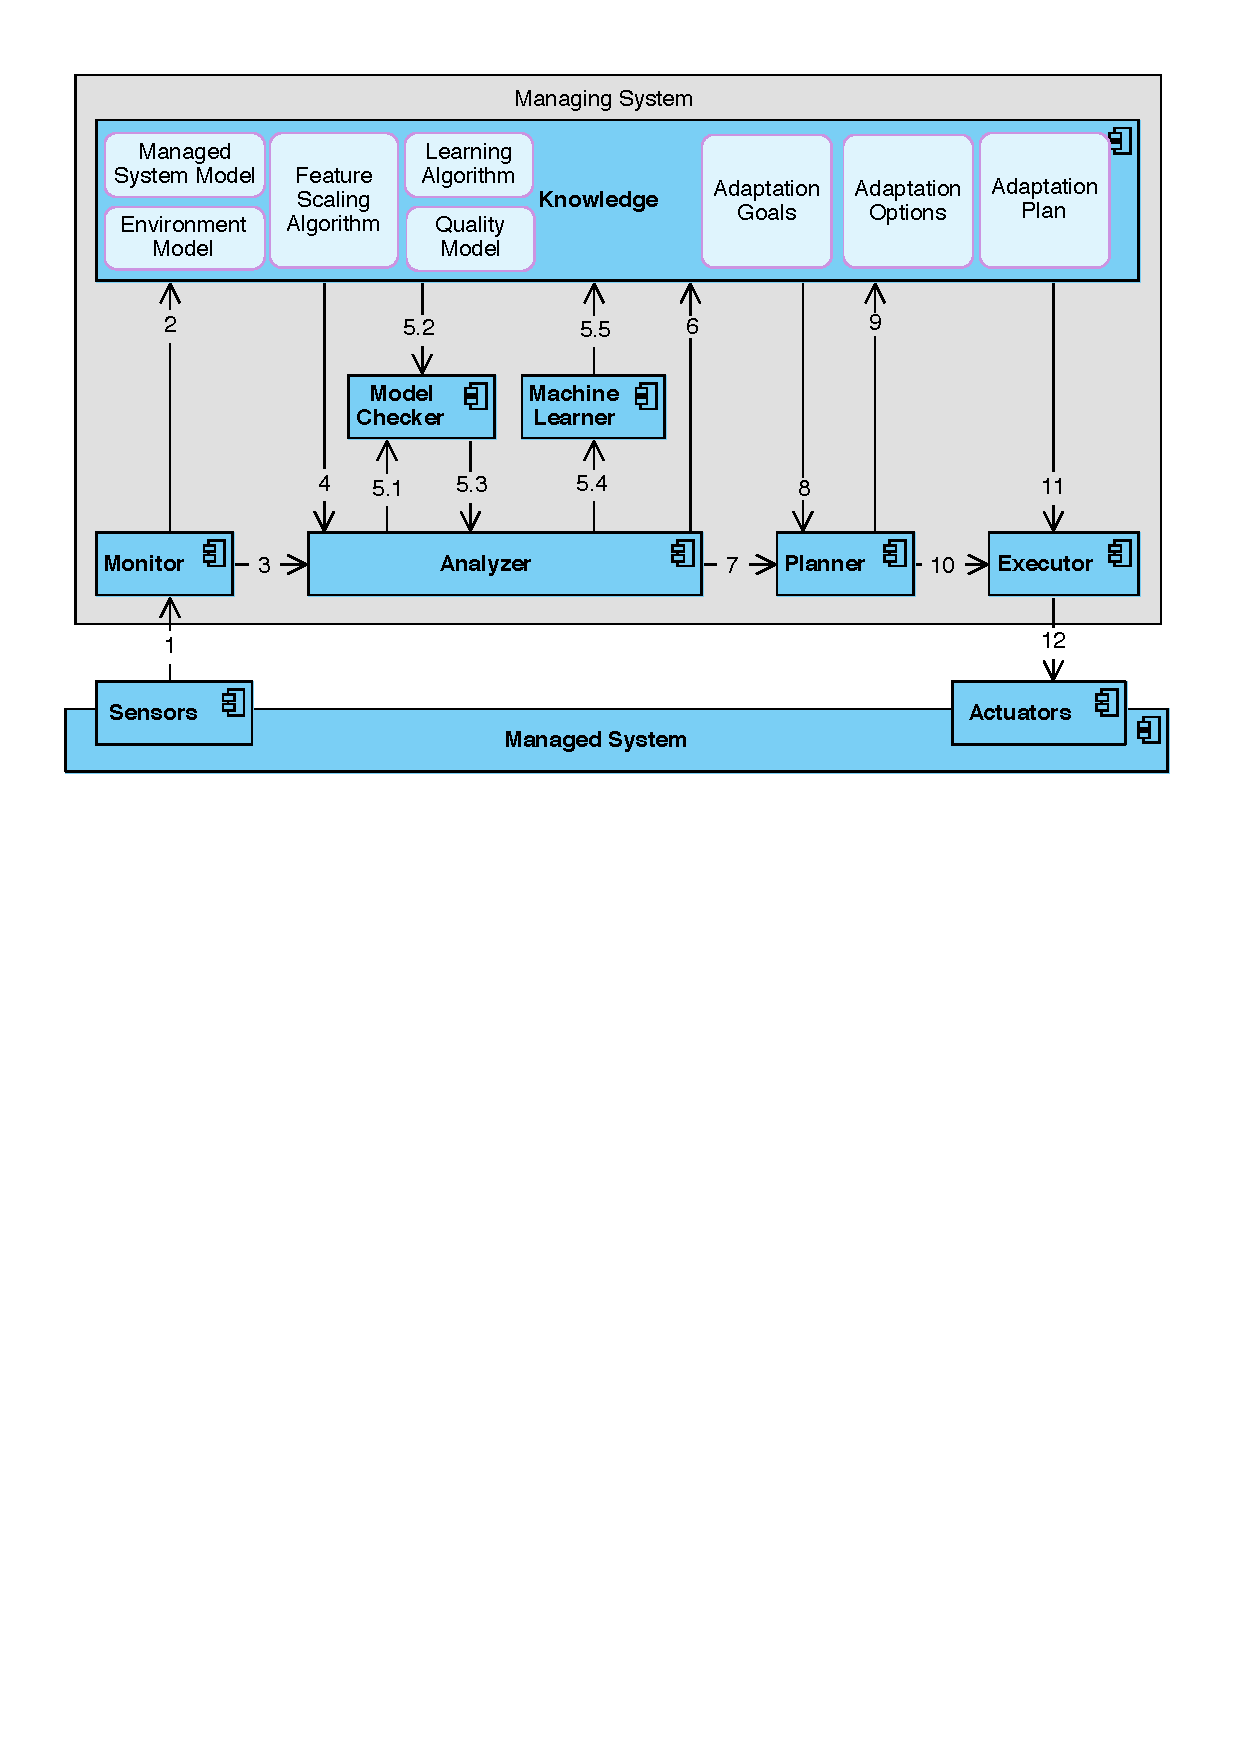
\includegraphics[keepaspectratio, width=\linewidth]{figures/TrainingView.pdf}
	\caption{Training phase in self-adaptive systems}
	\label{TrainingView}
\end{figure}
The flow of the monitor, planner and executor components is the same as in ActivFORMS, see section \ref{Activforms}. Therefore, we start with the analyzer. (4) the analyzer reads the adaptation options and the current uncertain values of the managed system and its environment. (5.1) then it sends this data to the model checker. (5.2) the model checker reads a corresponding quality model and simulate it with each adaptation option for estimating the values of the quality requirements. (5.3) then it sends the estimated values back to the analyzer. (5.4) first, the analyzer updates the placeholders of the adaptation options with the corresponding estimated values. Then the analyzer sends the verified adaptation options and current uncertain values to the machine learner in the form of a training dataset. (5.5) the machine learner uses the feature scaling algorithm to rescale the features values in the training dataset and then train the learning algorithm on that dataset. (6) then the analyzer determines whether the current adaptation option is able to accomplish the adaptation goals. (7) if the current adaptation option is unable to accomplish the adaptation goals, the analyzer triggers the planner.

Similarly, figure \ref{TestingView} shows the flow of our approach during the testing phase in self-adaptive systems. 
\begin{figure}[H]
	\centering
	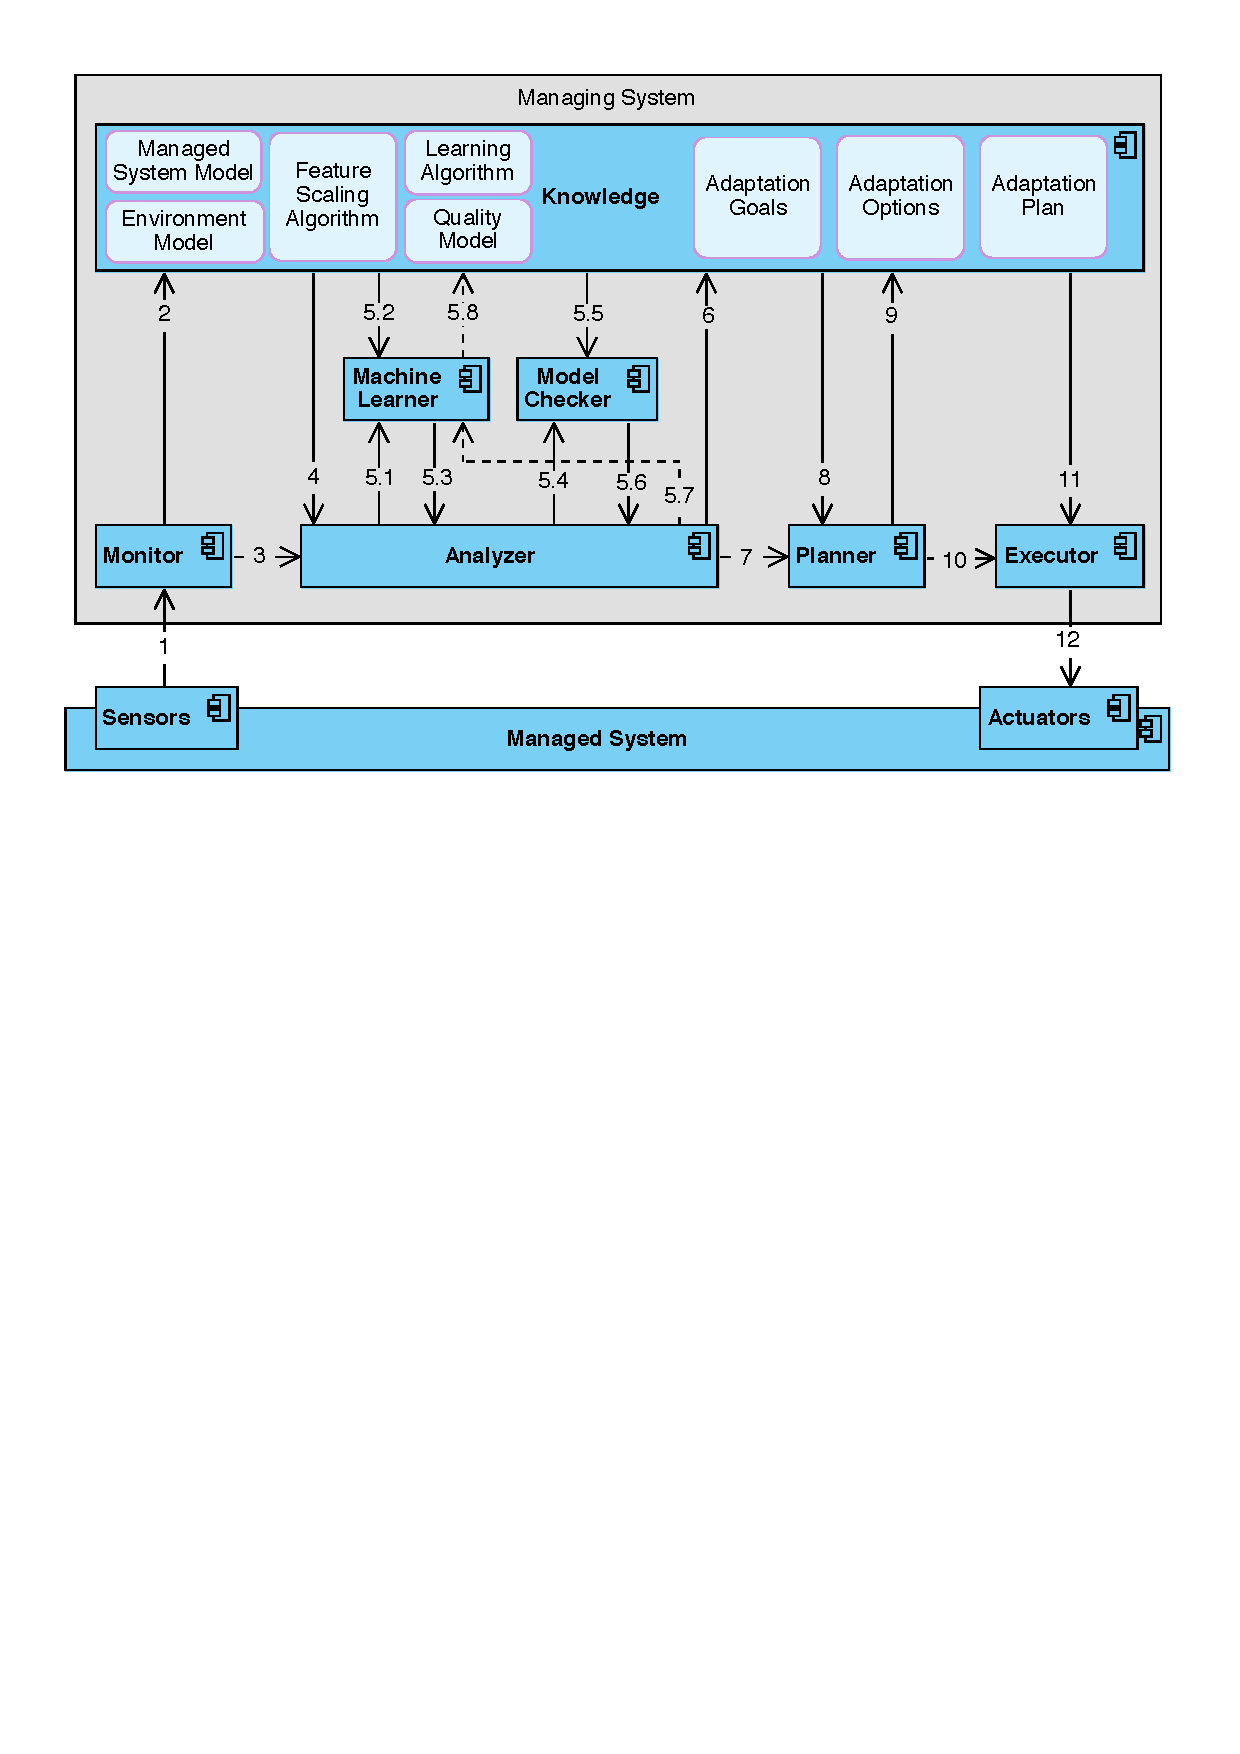
\includegraphics[keepaspectratio, width=\linewidth]{figures/TestingView.pdf}
	\caption{Testing phase in self-adaptive systems}
	\label{TestingView}
\end{figure}
Again we start with the analyzer component. (4) the analyzer reads the adaptation options and current uncertain values of the managed system and its environment. (5.1) then it sends this data to the machine learner in the form of a testing dataset. (5.2) the machine learner uses the feature scaling algorithm to rescale the features values in the testing dataset. In addition, it uses the learning algorithm to predict the values of the quality requirement(s) for each adaptation option. (5.3) then it sends the predicted values back to the analyzer. (5.4) first, the analyzer uses the predicted values to select the relevant adaptation options which fulfill the quality requirement(s). If there are no such adaptation options, it selects all the available adaptation options. Then it sends the selected adaptation options and the current uncertain values to the model checker. (5.5) the model checker reads a corresponding quality model and simulate it with each selected adaptation option for estimating the values of the quality requirements. (5.6) then it sends the estimated values back to the analyzer. (5.7) first, the analyzer updates the placeholders of the selected adaptation options with the corresponding estimated values. Here, the testing phase intermixes with the training phase. The analyzer then sends the verified adaptation options and the current uncertain values to the machine learner in the form of a training dataset. (5.8) the machine learner uses the feature scaling algorithm to rescale the features values in the training dataset and train the learning algorithm on that dataset. (6) then the analyzer determines whether the current adaptation is able to accomplish the adaptation goals. (7) if the current adaptation option is unable to accomplish the adaptation goals, the analyzer triggers the planner.
\newpage
\section{Implementation} \label{Implementation}
In this section, we present the implementation of our approach with online supervised learning on DeltaIoT. We used an open source machine learning library called Scikit-Learn \cite{SLMLIP-2011} for the implementation. We start by explaining the settings of the simulator and model checking. Then we present the implementation of the preprocessing which includes data preprocessing, feature selection, feature scaling, and model selection. Similarly, in the end, we present the implementation of the training and testing phases.
\subsection{Settings} \label{Settings}
Recall that the simulator provided by DeltaIoT allows to manage the uncertainties and distribution of the packets. We used the profiles of uncertainties provided by DeltaIoT for managing the uncertainties. In addition, some constant values are also used. The profiles of uncertainties represent the fluctuation of the traffic load of the motes and SNR in the environment. These profiles contain the real data for 12 hours. The simulator repeats these profiles in 12 hour intervals. The fluctuation of the traffic load is set to 100\% for the motes 3, 8, 9 and 15, whereas it is 50\% for the motes 2, 4, 5, 6, 7, 11, 12 and 14. The profiles of uncertainties are used to set the fluctuation of the traffic load for the motes 10 and 13. Similarly, the profiles of uncertainties are used to set the SNR between the motes 10 and 6, and motes 12 and 3, see figure \ref{Profiles}.
\begin{figure}[H]
	\centering
	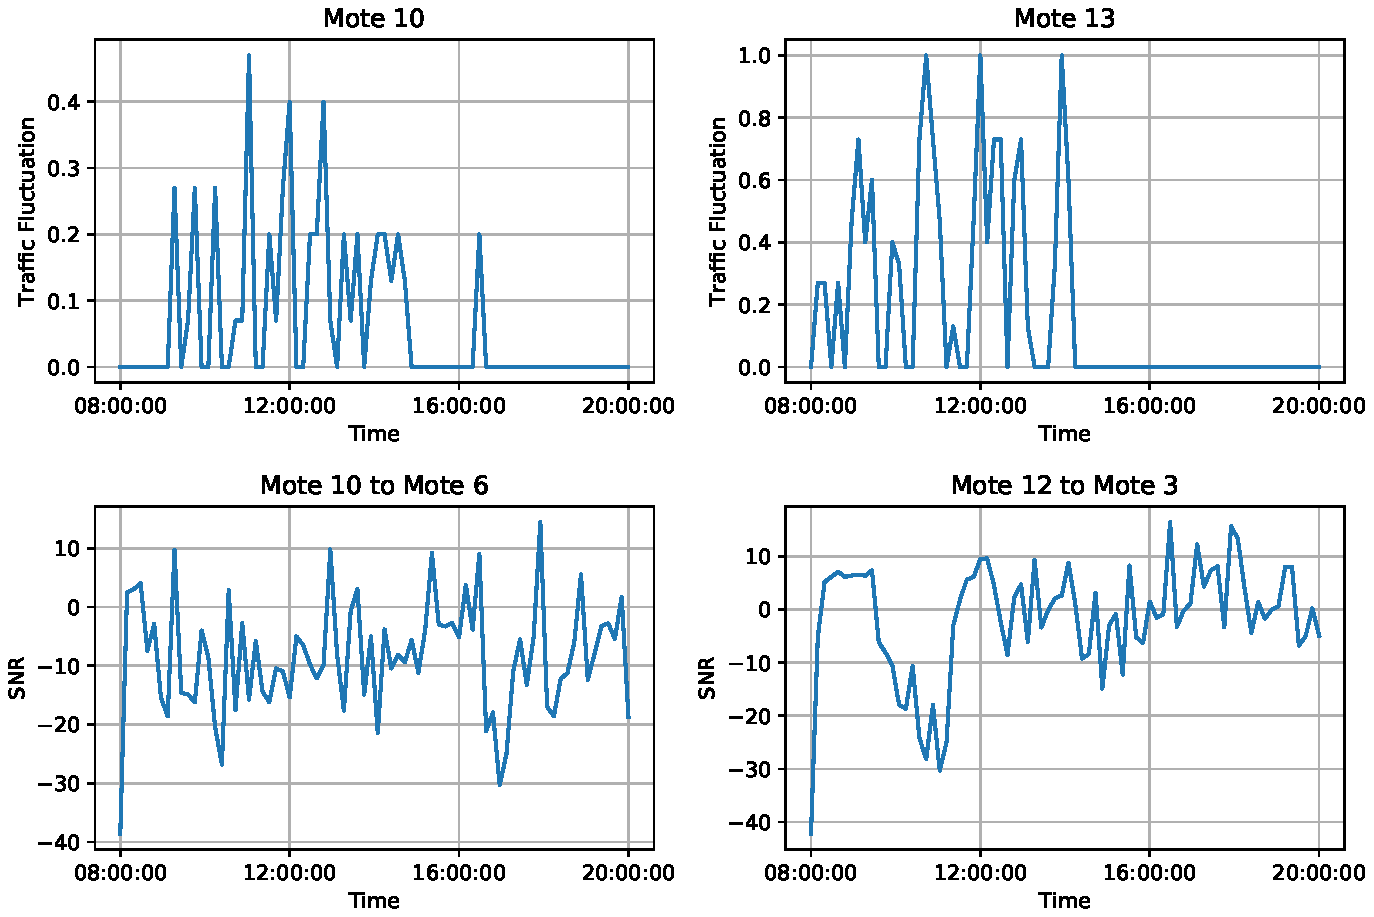
\includegraphics[keepaspectratio, width=\linewidth]{graphs/Profiles.pdf}
	\caption{Profiles of uncertainties}
	\label{Profiles}
\end{figure}
The distribution of the packets among the parents motes are set with a difference of 20\%, i.e., 0/100, 20/80, 40/60, 60/40, 80/20, 100/0. Recall that  DeltaIoT has 3 motes (mote 7, 10, and 12) with two parents. Therefore, this distribution gave us 216 adaptations options in total, i.e., 6 x 6 x 6 = 216.

In the section \ref{Method}, we defined three independent variables (ActivFORMS, classification and regression approaches) which will be used in the experiments. In these approaches, we use a statistical model checker to estimate the quality requirements. For the packet loss quality requirement, the accuracy of the statistical model checker is set to 99\% with a confidence of 90\%. The statistical model checker uses this accuracy and confidence to automatically compute the required number of simulations. For energy consumption quality requirement, the statistical model checker uses 30 simulations which is determined to be equal to 5\% RSEM (Relative standard error of mean) %\cite{AMBATESASWG-2017}. 
\subsection{Preprocessing}
In this section, we present the implementation of the preprocessing in the context of DeltaIoT. We ran the simulator with ActivFORMS for 12 hours for collecting the raw data of 76 adaptation cycles. There are 216 adaptation decisions in each adaptation cycle. In total there are 16416 adaptation decisions. Each adaptation decision includes the configurations of the motes, SNR and traffic load of the motes (uncertain values), and a packet loss (quality requirement), see listing \ref{RawData}.
\begin{lstlisting}[language=json, caption=An overview of the raw data, label=RawData]
{
	"adaptation_cycles": [
		{
			"adaptation_decisions": [
				...
				{
					"packet_loss": 6,
					"energy_consumption": 1266,
					"motes_configurations": [
						...
						{
							"id": 7,
							"load": 10,
							"energy_level": 11877,
							"parents": 2,
							"queue_size": 0,
							"traffic_load": 50,
							"links": [
								{
									"source_id": 7,
									"destination_id": 2,
									"power": 15,
									"packets_distribution": 0,
									"snr": 1
								},
								{
									"source_id": 7,
									"destination_id": 3,
									"power": 15,
									"packets_distribution": 100,
									"snr": -2
								}
							]
						},
						{
							"id": 8,
							"load": 10,
							"energy_level": 11877,
							"parents": 1,
							"queue_size": 0,
							"traffic_load": 100,
							"links": [
								{
									"source_id": 8,
									"destination_id": 1,
									"power": 15,
									"packets_distribution": 100,
									"snr": 1
								}
							]
						},
						...
					]
				},
				...
			]
		},
		....
	]
}
\end{lstlisting}
\subsubsection{Data Preprocessing}
Recall that in data preprocessing the raw data is first cleaned by using the domain knowledge and then converted into a dataset. As we can see that the collected raw data has many unwanted values such as energy consumption, mote id, energy level, power, etc. Recall that the packet loss quality requirement is affected by the values of SNR, packets distribution and traffic load. Therefore, by using this domain knowledge we removed all the unwanted values from the raw data, see listing \ref{CleanRawData}.
\begin{lstlisting}[language=json, caption=An overview of the raw data after removing the unwanted values, label=CleanRawData]
{
	"adaptation_cycles": [
		{
			"adaptation_decisions": [
				{
					"packet_loss": 6,
					"motes_configurations": [
						...
						{
							"traffic_load": 50,
							"links": [
								{
									"packets_distribution": 0,
									"snr": 1
								},
								{
									"packets_distribution": 100,
									"snr": -2
								}
							]
						},
						{
							"traffic_load": 100,
							"links": [
								{
									"packets_distribution": 100,
									"snr": 1
								}
							]
						},
						...
					]
				},
				...
			]
		},
		....
	]
}
\end{lstlisting}
Now the raw data needs to be converted into the datasets which work with classification and regression approaches. The datasets we made for these approaches contain same features, i.e., SNR, packets distribution and traffic load. For regression, the targets are real values of packet loss. In contrast, the classification has class 0 when the packet loss is >=10\%, and class 1 when it is <10\%, see tables \ref{DeltaIoTClassification} and \ref{DeltaIoTRegression}.
\begin{table}[H]
	\centering
	\begin{tabular}{c|c|c|c|c}
		\hline
		\multicolumn{1}{c|}{} & \multicolumn{3}{c|}{\textbf{Features}} & \multicolumn{1}{c}{\textbf{Target}} \\
		\cline{1-1} \cline{2-4} \cline{5-5}
		\multicolumn{1}{c|}{Item} & \multicolumn{1}{c|}{SNR} & \multicolumn{1}{c|}{Packets Distribution} & \multicolumn{1}{c|}{Traffic Load} & \multicolumn{1}{c}{Packet Loss} \\
		\cline{1-1} \cline{2-2} \cline{3-3} \cline{4-4} \cline{5-5}
		1 & 3, 1, 0, ... & 100, 100, 100, ... & 50, 100, 50, ... & 1 \\
		\hline
		2 & 2, 1, -1, ... & 100, 100, 100, ... & 50, 100, 50, ... & 0 \\
		\hline
		3 & 2, 0, -1, ... & 100, 100, 100, ... & 50, 100, 50, ... & 0 \\
		\hline
	\end{tabular}
	\caption{Dataset for classification}
    \label{DeltaIoTClassification}
\end{table}
\begin{table}[H]
	\centering
	\begin{tabular}{c|c|c|c|c}
		\hline
		\multicolumn{1}{c|}{} & \multicolumn{3}{c|}{\textbf{Features}} & \multicolumn{1}{c}{\textbf{Target}} \\
		\cline{1-1} \cline{2-4} \cline{5-5}
		\multicolumn{1}{c|}{Item} & \multicolumn{1}{c|}{SNR} & \multicolumn{1}{c|}{Distribution} & \multicolumn{1}{c|}{Traffic} & \multicolumn{1}{c}{Packet Loss} \\
		\cline{1-1} \cline{2-2} \cline{3-3} \cline{4-4} \cline{5-5}
		1 & 3, 1, 0, ... & 100, 100, 100, ... & 50, 100, 50, ... & 6 \\
		\hline
		2 & 2, 1, -1, ... & 100, 100, 100, ... & 50, 100, 50, ... & 16 \\
		\hline
		3 & 2, 0, -1, ... & 100, 100, 100, ... & 50, 100, 50, ... & 11 \\
		\hline
	\end{tabular}
	\caption{Dataset for regression}
	\label{DeltaIoTRegression}
\end{table}
Each item in the datasets represents an adaptation decision and has 48 features (17 SNR, 17 packets distribution, and 14 traffic load) and one target. The features show the configurations of the 14 motes. The reason for 17 SNR and packet distribution is the three motes with two parents.
\subsubsection{Feature Selection}
Both of the datasets which we made in data preprocessing have a high number of features, i.e., 48. Therefore, we used a tree-based feature selection algorithm to select the most useful features, see appendix \ref{FeatureSelectionAlgorithms}. Figure \ref{FeatureSelection} shows the importance of each feature for finding the packet loss quality requirement.
\begin{figure}[H]
    \centering
    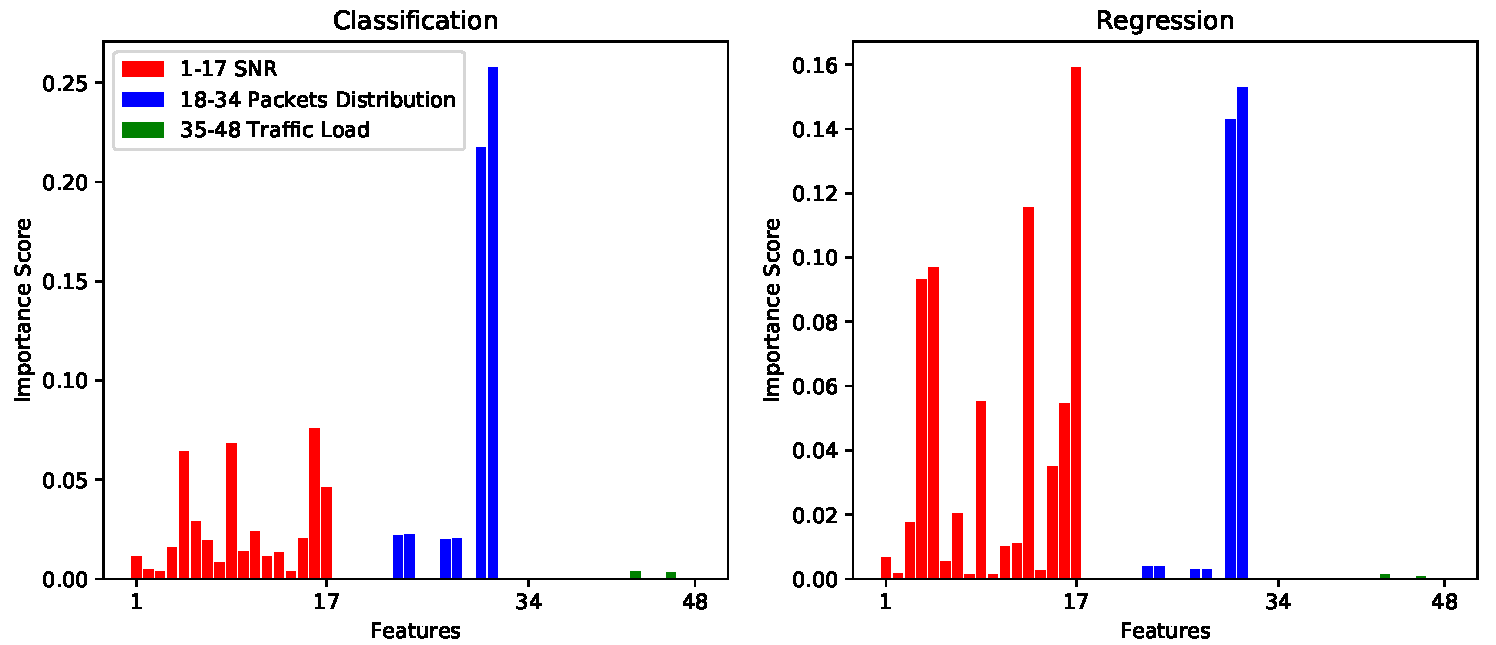
\includegraphics[keepaspectratio, width=\linewidth]{graphs/FeatureSelection.pdf}
    \caption{The importance of the features for classification and regression}
    \label{FeatureSelection}
\end{figure}
The tree-based algorithm has selected the same subset for both approaches. However, their importance score is different. Therefore, we applied the domain knowledge to verify both of the subsets. There are 25 features in both subsets, i.e., 17 SNR, 6 packets distribution and 2 traffic load. The remaining 23 features are not present in the subsets. It may be due to their constant values which we assigned while setting up the simulator, see section \ref{Settings}. Hence, it is clear from the domain knowledge that the selected subsets have all the required features which are subject to change. Table \ref{SelectedFeatures} shows the features present in the selected subsets.
\begin{table}[H]
    \centering
    \begin{tabular}{c|ccccccccccccccc}
        \hline
        \multicolumn{1}{c}{\textbf{Features}} & \multicolumn{14}{|c}{\textbf{Mote's Id}} \\
        \cline{1-2} \cline{3-15}
        & 2 & 3 & 4 & 5 & 6 & 7* & 8 & 9 & 10* & 11 & 12* & 13 & 14 & 15 \\
        \hline
        SNR & \checkmark & \checkmark & \checkmark & \checkmark & \checkmark & \checkmark & \checkmark & 
        \checkmark & \checkmark & \checkmark & \checkmark & \checkmark & \checkmark & \checkmark \\
        \hline
        Packets Distribution & & & & & & \checkmark & & & \checkmark & & \checkmark & & & \\
        \hline
        Traffic Load & & & & & & & & & \checkmark & & \checkmark & & & \\
        \cline{1-15}
        \multicolumn{15}{c}{*motes with two parents}
    \end{tabular}
    \caption{The most useful features for classification and regression}
    \label{SelectedFeatures}
\end{table}
\subsubsection{Feature Scaling and Model Selection}
Recall that feature scaling is mostly used when there are big differences between the features values. The features which we selected in feature selection process have big differences, e.g., SNR = -2, distribution = 100, and traffic = 50. Therefore, we used min-max, max-abs and standardization feature scaling algorithms to rescale the features values, see appendix \ref{FeatureScalingAlgorithms}. Figure \ref{FeatureScaling} shows how these algorithms rescaled the features values.
\begin{figure}[H]
    \centering
    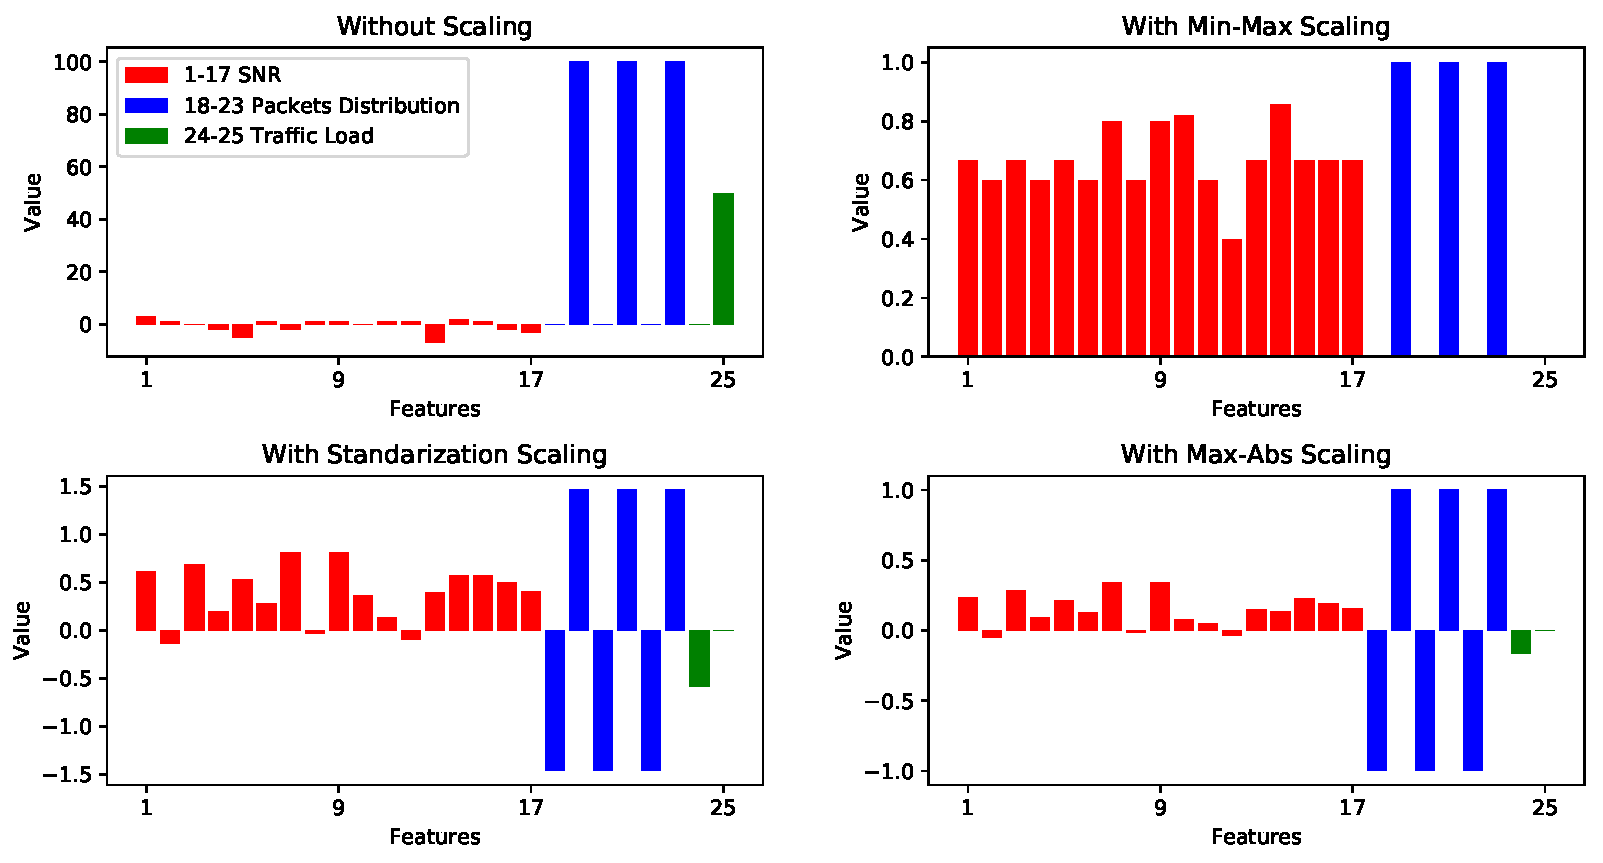
\includegraphics[keepaspectratio, width=\linewidth]{graphs/FeatureScaling.pdf}
    \caption{Feature scaling with min-max, max-abs and standardization}
    \label{FeatureScaling}
\end{figure}
The top left bar graph in the figure shows the original values of the features. The other bar graphs show the rescaled values of the features with respective feature scaling algorithm. In order to find the suitable feature scaling algorithm, we combined the feature scaling process with the model selection process.

We selected three learning algorithms named as Stochastic Gradient Descent (SGD), Perceptron, and Passive-Aggressive (PA) in the model selection process, see appendix \ref{LearningAlgorithms}. In addition, we also set up two learning goals, see table \ref{LearningGoals}
\begin{table}[H]
	\centering
	\begin{tabular}{|p{1cm}|p{11cm}|}
		\hline
		\textbf{LG1} & The error rate should be less than <5\% \\
		\hline
		\textbf{LG2} & The training cycles to achieve this error rate should be minimum \\
		\hline
	\end{tabular}
	\caption{Learning Goals}
	\label{LearningGoals}
\end{table}
The selected learning algorithms have various hyperparameters which can be configured. However, we only configured their loss and penalty (regularization) parameters. The loss parameter is used to minimize the loss between the actual and predicted target. The penalty parameter is used to reduce over-fitting \cite{MMLWSL-2014}.

For selecting the desired learning algorithms for classification and regression approaches, the datasets with rescaled features are divided into 5 different training and testing sizes, e.g., 15 cycles training and 65 cycles testing, 30/45, 45/30, 60/15, and 70/10. Each learning model is trained and tested for 20 times on each of the sizes in order to achieve reliable results. 

For classification, SGD uses 5 types of losses and 3 types of penalties, i.e., 15 instances. Perceptron only uses 3 types of penalties, and PA uses 2 types of losses. First, we tested 15 instances of SGD and selected the best one, see appendix \ref{SGDClassifiersTests}. Then we tested the selected SGD with 3 instances of Perceptron and 2 instances of PA, see figure \ref{Classifiers}.
\begin{figure}[H]
    \centering
    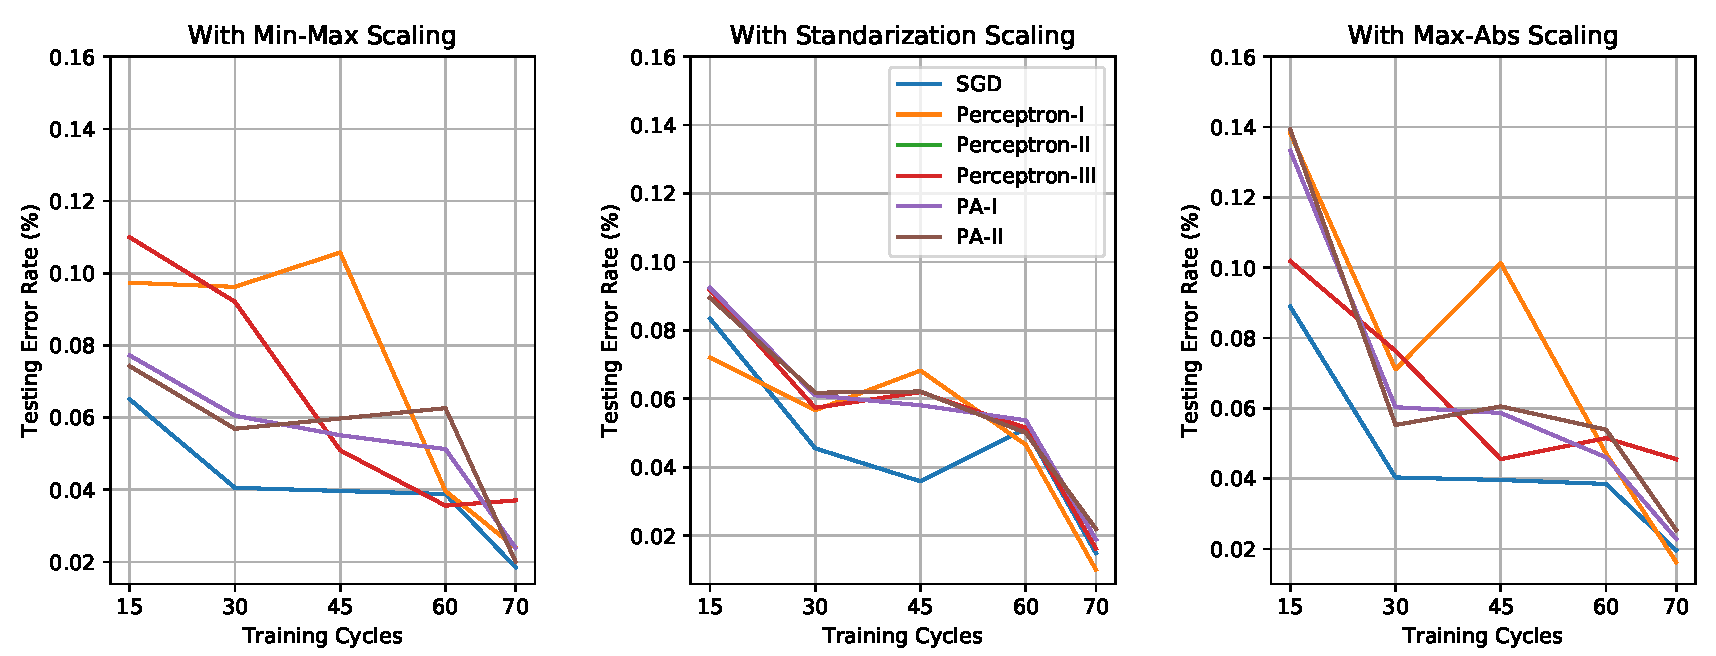
\includegraphics[keepaspectratio, width=\linewidth]{graphs/ClassificationModelSelection.pdf}
    \caption{Performance of the instances of the learning algorithms for classification}
    \label{Classifiers}
\end{figure}
The above figure shows that SGD fulfilled the learning goals with min-max and max-abs feature scaling algorithms. However, only one needs to be selected. Therefore, we selected SGD with min-max because the initial testing error rate of SGD was lower compared to max-abs. The configurations of the hyperparameters are given in appendix \ref{Hyperparameters}. The figure also shows that SGD requires 30 adaptation cycles, i.e. 6480 items, to achieve the learning goals. Therefore, in training phase, we will initially train the SGD on 30 cycles.

For regression, SGD uses 4 types of losses and 3 types of penalties, i.e., 12 instances. In Scikit-Learn, Perceptron is not able to work with regression. PA uses 2 types of losses. Again we first tested the 12 instances of SGD and selected the best one, see appendix \ref{SGDRegressorsTests}. Then the selected SGD is tested with 2 instances of PA, see figure \ref{Regressors}. 
\begin{figure}[H]
    \centering
    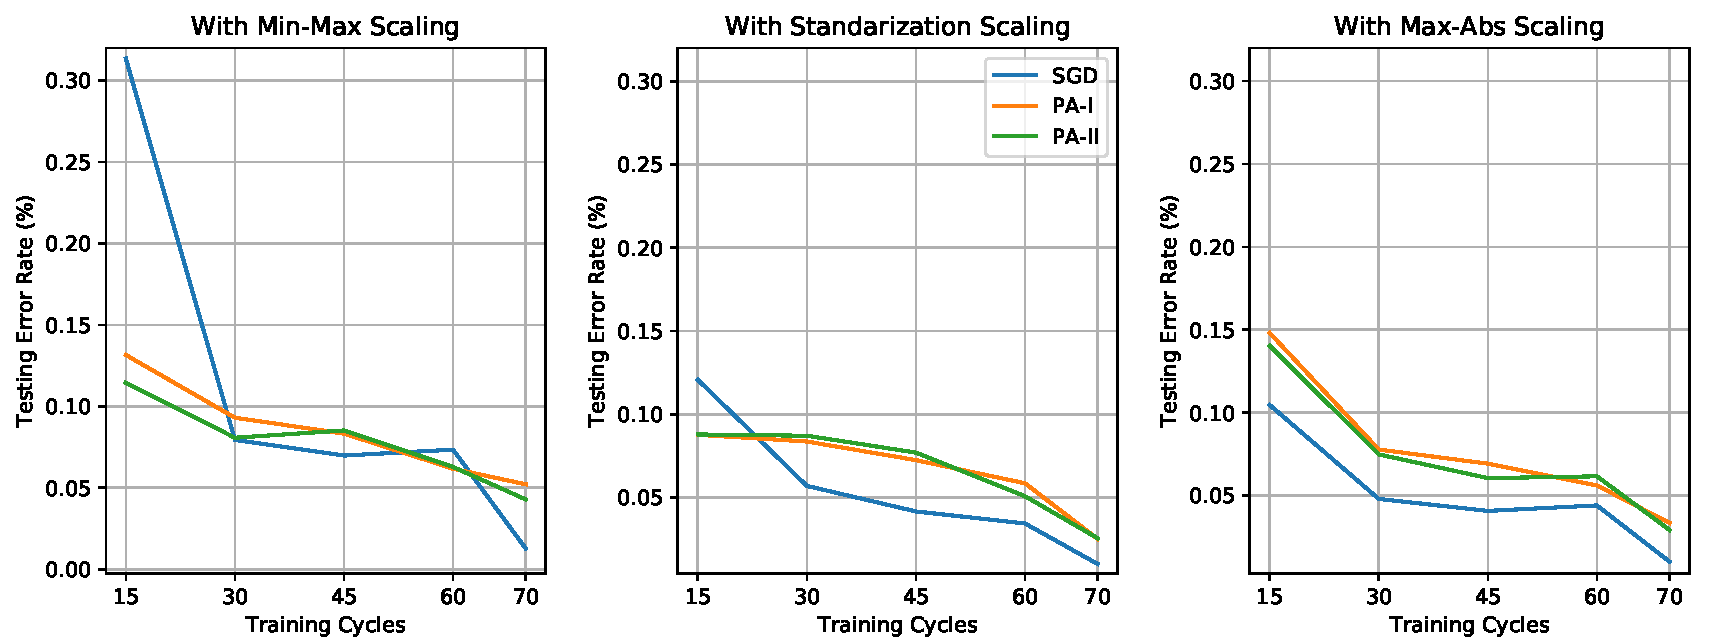
\includegraphics[keepaspectratio, width=\linewidth]{graphs/RegressionModelSelection.pdf}
    \caption{Performance of the instances of the learning algorithms for regression}
    \label{Regressors}
\end{figure}
It is clear from the above figure that SGD fulfilled the learning goals with max-abs feature scaling algorithm. Therefore, we selected these algorithms. The configurations of the hyperparameters are given in appendix \ref{Hyperparameters}. The figure also shows that SGD needs 30 adaptation cycles to achieve the learning goals. Therefore, we will initially train the SGD on 30 cycles during the training phase.
\subsection{Training and Testing}
Figure \ref{DeltaIoTTrainingTestingView} shows an overview of DeltaIoT in the training and testing phases. 
\begin{figure}[H]
    \centering
    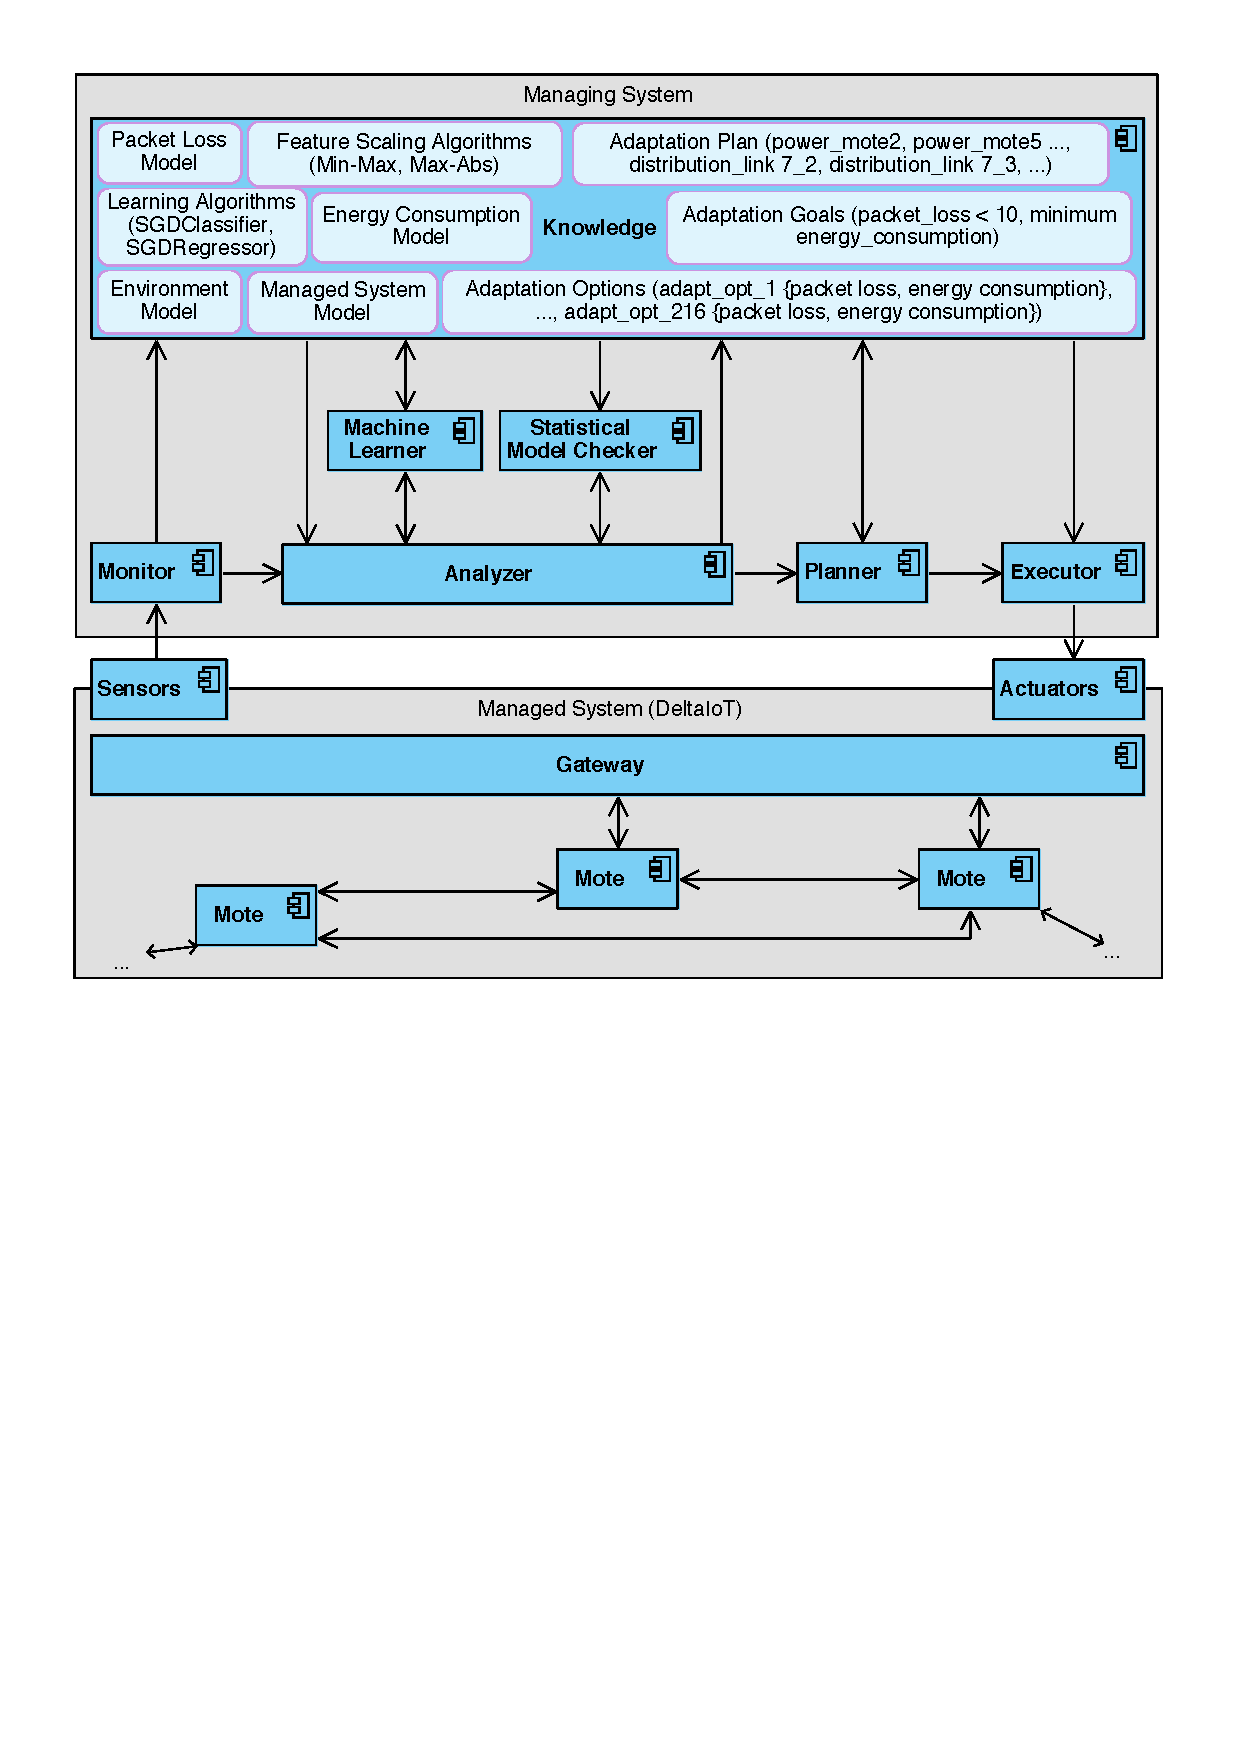
\includegraphics[keepaspectratio, width=\linewidth]{figures/DeltaIoTTrainingTestingView.pdf}
    \caption{An overview of the training and testing phases in DeltaIoT}
    \label{DeltaIoTTrainingTestingView}
\end{figure}
The selected learning and feature scaling algorithms are placed in the repository. SGD classifier and min-max work with classification, and SGD regressor and max-abs with regression. During the initial training phase, the learning algorithms are trained on 30 adaptation cycles. Packet loss and energy consumption models are the quality models. The managed system model represents DeltaIoT and environment model represents the environment in which DeltaIoT operates. These runtime models holds SNR, traffic load and current values of the quality requirements. The adaptation plan consists of adaptation actions such as change the power of mote 2 from 15 to 14, change the distribution of the packets between mote 7 and 2 from 80\% to 40\%, etc. The adaptation goal includes the packet loss and energy consumption quality requirements. The adaptation options represent 216 different configurations (power, load, packets distribution, etc.) of 14 motes. The managed system is DeltaIoT which contains a gateway and a network of 14 motes. The actions of the remaining components are same as mentioned in the section \ref{TrainingAndTesting}.
\newpage
\section{Results and Analysis} \label{ResultsAndAnalysis}
In this section, we show the results of the two controlled experiments which we explained in section \ref{Method}. We begin with the first experiment which compares the approaches (ActivFORMS, classification, and regression). Then we present the second experiment which compares the adaptation options selected by the approaches. In the end, we discuss the results. The experiments are conducted on the simulator provided by DeltaIoT. For simulation, we used MacBook Air with 1.6 GHz Core i5 processor and 4 GB 1600MHz DDR3 RAM. The settings of the simulator and model checking are the same as mentioned in section \ref{Settings}. 
\subsection{Comparison of the Approaches}
In the first experiment, we independently ran ActivFORMS, classification, and regression. With each approach, we ran the simulator for 300 adaptation cycles that is equal to 48 hours. However, during classification and regression, we initially trained the learning algorithms on first 30 adaptation cycles and then started the testing. Figure \ref{Comparison} shows the results of these approaches from 31-300 adaptation cycles.
\begin{figure}[H]
    \centering
    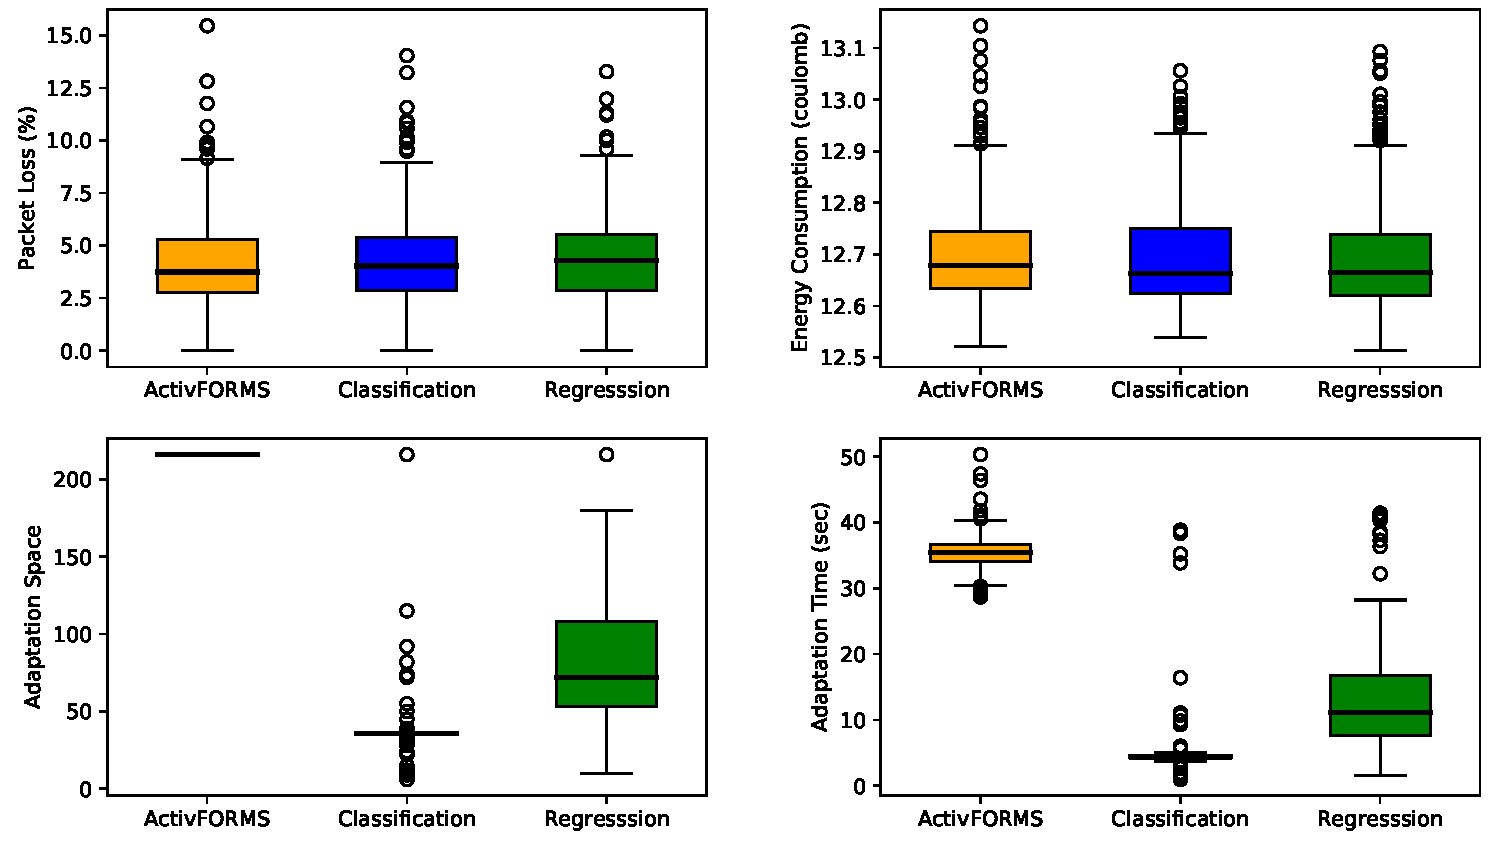
\includegraphics[keepaspectratio, width=\linewidth]{graphs/Comparison.pdf}
    \caption{Comparison of the approaches}
    \label{Comparison}
\end{figure}
It is clear from the above figure that all the approaches achieved the quality requirements, i.e., packet loss <10\%, and minimum energy consumption. On average, the packet loss is  4.4\% for all of them. Similarly, the average energy consumption for all the approaches is  12.6 coulomb.

From the above figure, we can also see that ActivFORMS constantly explored all the available adaptation options (216) to accomplish the quality requirements. However, classification only explored 40 adaptation options on average. Hence, reduced the adaptation space by on average 81.2\% compared to ActivFORMS. Similarly, regression explored 90 adaptation options on average. It reduced the adaptation space by on average 58.3\% compared to ActivFORMS. The reduced adaptation space also helped classification and regression to decrease the adaptation time to on average 5.2 and 12.7 seconds respectively compared to ActivFORMS which took 34.8 seconds.

%\emph{Conclusion:} The research question of this thesis was to investigate how to reduce the adaptation space in self-adaptive systems using machine learning. Within this research question, we also aim to achieve the quality requirements of self-adaptive systems. To answer this question we particularly focused on online supervised learning with classification and regression approaches. The above results show that by combining classification or regression with a model checker we can reduce the adaptation space in self-adaptive systems. It is also clear from the above results that classification and regression achieved the same quality requirement as ActivFORMS. This concludes that the research question of this thesis is answered.
%\subsubsection{Comparison of Time}
The adaptation time of DeltaIoT with classification and regression also includes the training and prediction time of the learning algorithms at each adaptation cycle. We also measured this time separately. For this, we started the timer when the analyzer sent the request to the model checker and stopped the timer when the analyzer received the response, see figure \ref{TimeMeasurement}.
\begin{figure}[H]
	\centering
	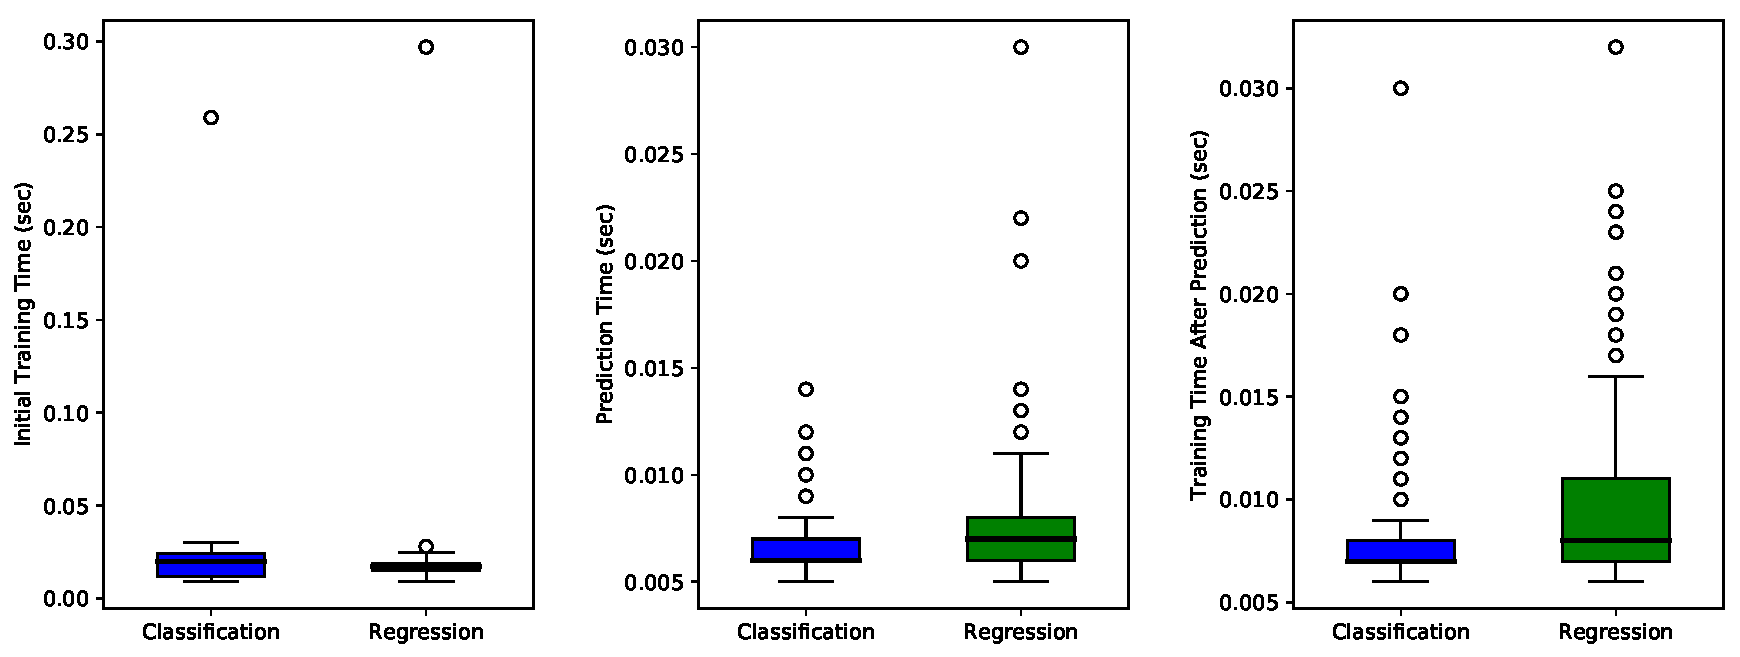
\includegraphics[keepaspectratio, width=\linewidth]{graphs/TimeMeasurement.pdf}
	\caption{Time measurements of classification and regression}
	\label{TimeMeasurement}
\end{figure}
We initially trained the learning algorithms on 30 adaptation cycles. The average initial training time is 0.02 and 0.03 seconds with classification and regression respectively. Similarly, the average prediction time with classification is 0.006 seconds, whereas with regression it is 0.007 seconds. The average training time after making the prediction is 0.008 and 0.010 seconds with classification and regression respectively. These results show that learning algorithms with both approaches took very less and similar time. This means that the learning algorithms have almost no overhead on the adaptation time.
\subsection{Comparison of the Selected Adaptation Options}
In the second experiment, we ran ActivFORMS, classification, and regression at the same time. The simulator again ran for 300 adaptation cycles. During this experiment, DeltaIoT was managed by ActivFORMS. At each adaptation cycle, ActivFORMS first analyzed the complete adaptation space. Then it compared its relevant adaptation options with the adaptation options selected by classification and regression. Again, we trained the learning algorithms on first 30 adaptation cycles and then started the testing. Figure \ref{OnlineLearning} shows the adaptation options selected by ActivFORMS compared to classification and regression.
\begin{figure}[H]
    \centering
    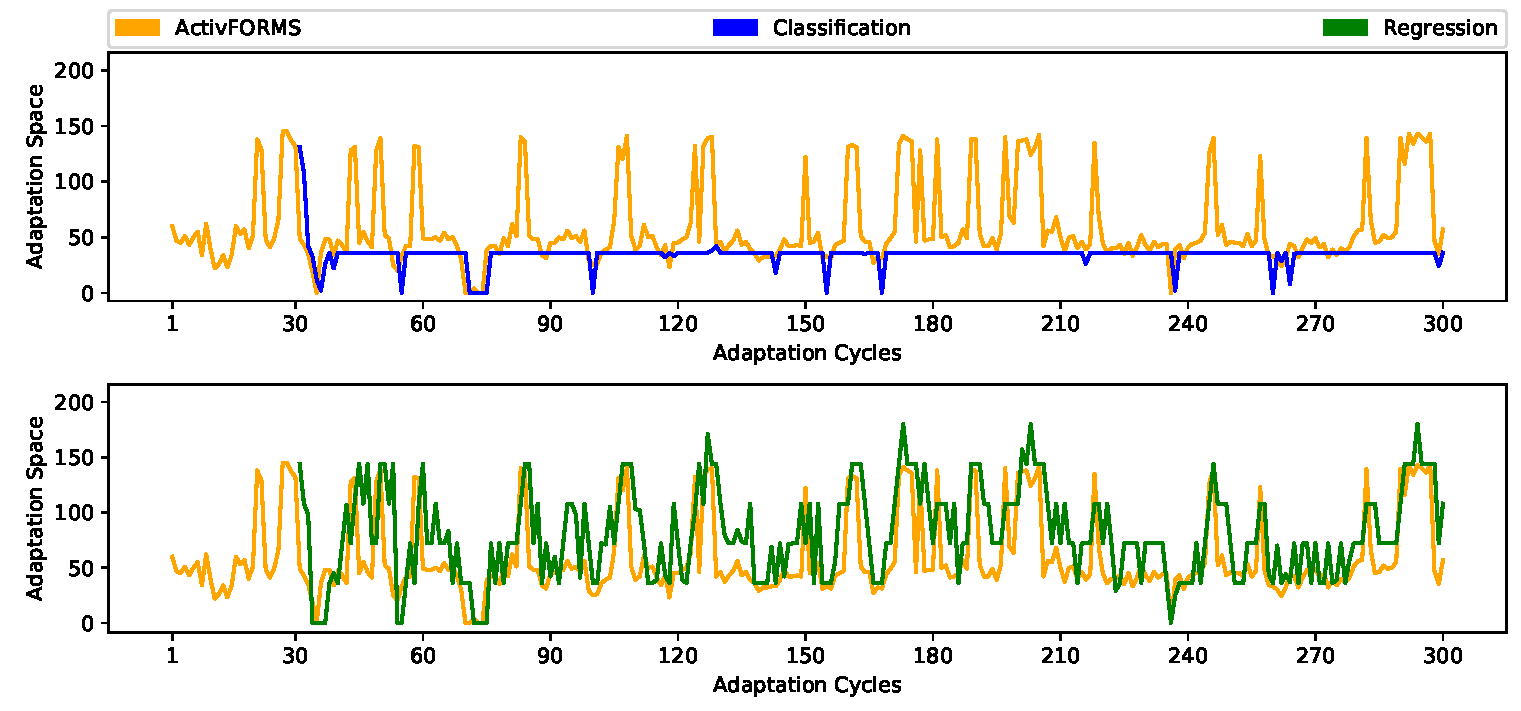
\includegraphics[keepaspectratio, width=\linewidth]{graphs/OnlineLearning.pdf}
    \caption{Comparison of the adaptation options selected by the approaches}
    \label{OnlineLearning}
\end{figure}
It is clear from the above figure that classification mostly selected a lower number of adaptation options than ActivFORMS throughout all the adaptation cycles. In contrast, regression selected mostly a higher number of adaptation options. This can be seen in detail in figure \ref{RelevantOptions}.
\begin{figure}[H]
    \centering
    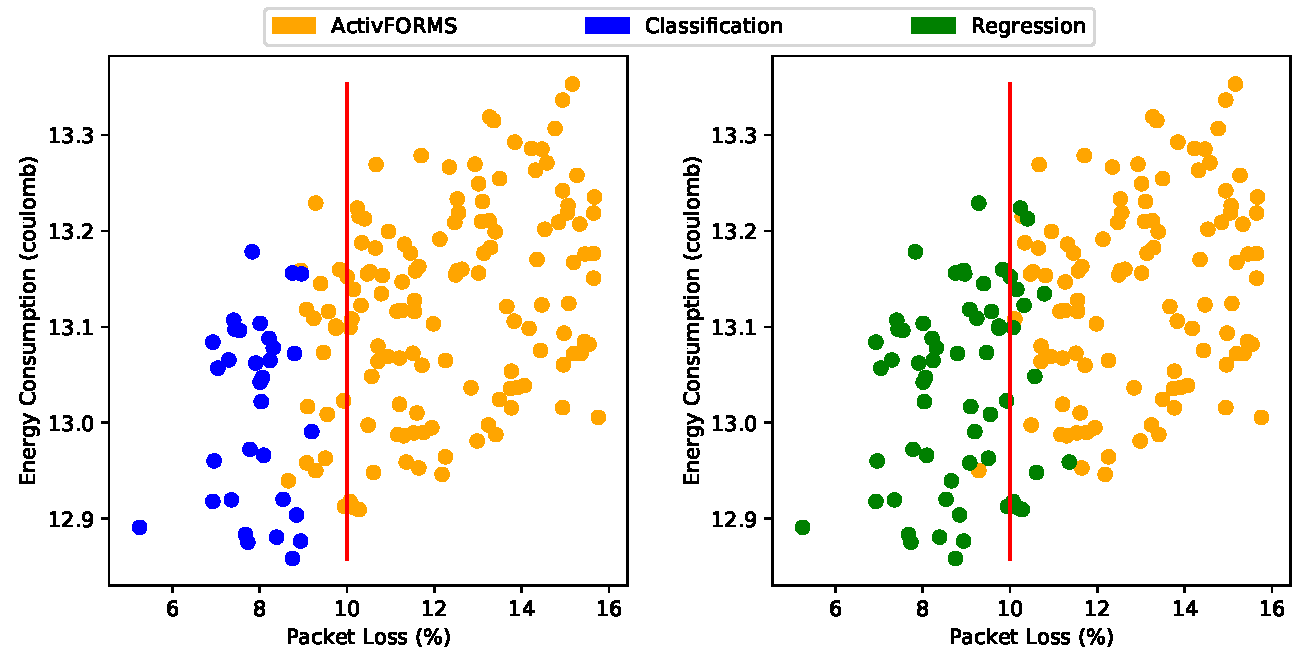
\includegraphics[keepaspectratio, width=\linewidth]{graphs/SelectedAdaptationOptions.pdf}
    \caption{Selection of the relevant adaptation options at a particular adaptation cycle}
    \label{RelevantOptions}
\end{figure}
The blue, orange and green dots represent the adaptation options selected by the respective approach. The red line separates the relevant adaptation options (on the left) from the irrelevant adaptation options (on the right). We can see that ActivFORMS analyzed all the available adaptation options. Whereas, classification selected a subset of the relevant adaptation options. On the other hand, regression selected most of the relevant adaptation options as well as a number of irrelevant options in addition. This shows that classification is more efficient than regression in terms of finding the most relevant adaptation option.
\subsection{Discussion} \label{Discussion}
The research question of this thesis was to investigate how to reduce the adaptation space in self-adaptive systems using machine learning. Within machine learning, we particularly focused on online supervised learning with classification and regression approaches. The results show that by combining classification or regression with a model checker we can reduce the adaptation space in self-adaptive systems. This concludes that the research question of this thesis is answered.

We conclude that classification is much better than regression because it dramatically reduces the adaptation space and time. However, at runtime regression is more adaptive than classification. Still, this did not help regression to beat classification in terms of adaptation space and time. This shows that one can choose the approach based on adaptivity or speed factor. However, this factor does not affect the quality requirements. The reason is that regression selects a subset of the adaptation options which contains slightly more adaptation options than needed. In contrast, classification selects fewer but more relevant. Therefore, the subsets selected by both approaches do contain the best adaptation option. 

Learning in an uncertain environment is a challenge. However, we show that online learning is very effective in this scenario as it continuously updates the learning algorithms. The learning algorithms used in classification and regression are significantly fast in the training and testing phases. This show that the learning algorithms have almost no overhead on the adaptation time. We believe that preprocessing plays a big role in this. On the other hand, this also shows that adaptation time is still somehow dependent on the computational speed of the model checker. Therefore, the configuration of the model checker must be optimally configured to reduce the adaptation time.

There are some drawbacks of online supervised learning. The preprocessing can be time consuming for large scale self-adaptive systems. In the case, if new adaptation options are added after applying online supervised learning, it might require to repeat the preprocessing. The reason is that in classification and regression we select the learning algorithms based on the current available adaptation options. Therefore, new adaptation options may reduce the accuracy of the learning algorithms. The selection of the relevant adaptation option is highly dependent on the accuracy of the learning algorithms. Therefore, lower accuracy can lead to undesired results. Moreover, we have not verified the scalability of our approach. Therefore, we are unaware of the problems which can come with a large number of adaptation options.
\newpage
\section{Related Work} \label{RealtedWork}
In this section, we discuss the existing work related to our approach. Most of the approaches that applied machine learning used a configurable system which consists of many features or configuration options. Each configuration option can affect the system's functional and non-functional requirements. We call the performance of these systems depends on parameter values of these features \cite{CESFPPOCS-2015}. The machine learning is used to find the optimal configuration based on learning and sampling. In this section, we discuss these approaches briefly.

Many approaches used machine learning to find the optimal configuration. For example, \cite{AUAATOCOSPS-2016} propose an approach BO4CO that uses Bayesian learning techniques to find the optimal configuration in stream processing systems. \cite{PPOCSSBFL-2015} uses Fourier learning algorithm to predict software performance predictions with guaranteed accuracy and confidence levels. \cite{TMLBATOMR-2013} explores machine learning based performance models to auto-tune the configuration parameters of Hadoop MapReduce. The approach supports vector regression model (SVR) that has good accuracy and computationally efficient.

\cite{PIMFHCS-2015} propose an approach which combines machine learning and sampling heuristics to derives a performance-influence model for a given configurable system which describes all relevant influences of configuration options and their interactions. The approach reduces the solution space to a tractable size by integrating binary and numeric configuration options and incorporating the domain knowledge. \cite{ARLATOWSAC-2009} propose a reinforcement learning approach for autonomic configuration and reconfiguration of multi-tier web systems. The approach adapts the web system based on performance and workload by changing virtual machine configurations. The approach also reduced the learning time for online decisions using an efficient initialization policy. \cite{TLFIMPIHCS-2017} propose a cost-aware transfer learning method that learns accurate performance models for configurable software from other resources such as simulators, etc. The approach uses a regression model which learns the relationship between source and target using only a few samples taken from the real system, leading to faster learning period.

\emph{Conclusion}: Most of the existing approaches used machine learning with sampling and other techniques to find an optimal configuration and to learn about the possible effect of each configuration of the system. In our approach, we learn the effect from the model checker. First, in the training phase, the model checker provides an estimate of each configuration. After that when the machine learner is trained, it starts to provide possible configurations to the analyzer that suits best with the current settings of the environment. The analyzer then uses the model checker to verify only those configurations that are verified by the machine learner. Our approach performs the continuous learning by training the machine learner again for these configurations that are verified by the model checker. This way we keep the machine learner always active along the path which the system takes.
\newpage

\section{Conclusion and Future Work} \label{Conclusion}
In this thesis, we reduce the adaptation space in self-adaptive systems by using machine learning. The adaptation space is reduced in order to enable the existing formal approaches to achieve the adaptation goals by only analyzing the relevant adaptation options. For reducing the adaptation space, we present an approach which integrates machine learning and a model checker with the MAPE-K feedback loop. This integration enables machine learning to select a subset of the adaptation options which can be further verified by the model checker. We evaluate the approach on a self-adaptive IoT application and compare the results with an existing formal approach called ActivFORMS. The results show that our approach successfully reduced the adaptation space as well as accomplished the quality requirements of DeltaIoT. In addition, the reduced adaptation space also significantly drops the adaptation time compared to ActivFORMS. We conclude that our approach enables the existing formal approaches to speed up the adaptation process while having the same quality guarantees. In addition, the fast adaptation process also helps them to deal with large adaptation space.

Scalability is one of the most important directions for the future work. We evaluated our approach with 216 adaptation options. This number may be relatively small compared to large self-adaptive systems which may contain hundreds or even thousands of adaptation options. Therefore, we plan to investigate the scalability of our approach in the future.

The adaptation goals of self-adaptive systems are often based on various quality requirements. In this thesis, we applied machine learning to only on one quality requirement, i.e., packet loss. Therefore, in future, we aim to test our approach with more than one quality requirement. This might help to reduce the adaptation space even more because of the narrow selection procedure.

We applied our approach on DeltaIoT. In future, we plan to apply our approach on other self-adaptive systems such as Automated Traffic Routing Problem (ATRP), Tele Assistance System (TAS), Znn.com, etc. In this thesis, we used online supervised learning and compared the results with ActivFORMS. In future, we aim to use different machine learning scenarios, e.g., unsupervised learning, reinforcement learning, etc., with different approaches such as RQV. 
\newpage
\hypersetup{urlcolor=black} 
\bibliographystyle{IEEEtran}
\bibliography{referenser}
\newpage
\pagenumbering{Alph}
\setcounter{page}{1}
\appendix
\section{Appendix 1} \label{Appendix}
In this section, we explain the algorithms which we used for the implementation of our approach. For the implementation, we used an open source machine learning library called Scikit-Learn \cite{SLMLIP-2011}. The implementation can be found on \\ \url{https://github.com/sarpreetsingh3131/2dv50e}
\subsection{Feature Selection Algorithms} \label{FeatureSelectionAlgorithms}
We used a tree based feature selection algorithm in the feature selection process. According to the Scikit-Learn, tree-based feature selection algorithms use an ensemble method to compute the importance of each feature in the dataset. There are various ensemble methods such as extra-trees, random forest, etc. We used the extra-trees method which is also known as extremely randomized trees. This method predicts the target of an item by aggregating the predictions of a group of predictors. The group includes either one or more learning algorithms which are also known as an ensemble. Extra-trees is faster than other ensemble methods because it uses random thresholds for making ensemble for each feature. The other ensemble methods use the best possible thresholds which require more time \cite{HOMLWSLATF-2017}.

\subsection{Feature Scaling Algorithms} \label{FeatureScalingAlgorithms}
We used min-max, max-abs and standardization feature scaling algorithms in the feature scaling process. Min-max subtracts the feature value from the min feature value and then divides it with the max minus min feature value. The result value lies from 0 to 1. Max-abs works similar to min-max, however, it divides the feature value only with the max feature value. Therefore, the result value lies from -1 to 1. Standardization subtracts the feature value from the features mean value, and then divides it with the variance. The result value always have a zero mean and unit variance \cite{HOMLWSLATF-2017}, \cite{SLMLIP-2011}. 

\subsection{Learning Algorithms} \label{LearningAlgorithms}
We used Stochastic Gradient Descent (SGD), Perceptron, and Passive-Aggressive (PA) algorithms in the model selection process. These algorithms support online supervised learning. SGD \cite{HOMLWSLATF-2017} finds the optimal solutions for a problem by iteratively changing the parameters which minimize the loss. In each iteration, it selects a random item from the dataset and calculates the gradients based on it. Due to random selection, SGD is much faster to train and test on larger datasets. The other gradient descent algorithms, e.g., batch gradient descent, are slow because they compute the gradient by using the complete dataset. Perceptron \cite{MMLWSL-2014} is an error-driven algorithm which is inspired by neurons. It initializes the parameters with a small random value or zero, and due to error-driven learning if the prediction is incorrect the parameters are updated, otherwise, it continues to the next item. It is also able to work with larger datasets, however, in Scikit-Learn it is only able to work with classification approach. PA \cite{OPAA-2006} uses an aggressive strategy to overcome the constraint imposed by the current instance. It initializes the parameters with zero, and due to aggressive behavior if the prediction is wrong it updates the parameters with as much value as required. Like other algorithms, it is also able to work with larger datasets.
\section{Appendix 2}
In this section, we show the results of the experiments which were conducted to select the best hyperparameters of SGD in terms of achieving the learning goals (see table \ref{LearningGoals}). We only configured the loss and penalty parameters. However, we do not provide their details in this thesis. Therefore, we recommend the interested readers to review the details on the website of Scikit-Learn.
\subsection{The Selection of SGD for Classification} \label{SGDClassifiersTests}
\begin{figure}[H]
	\centering
	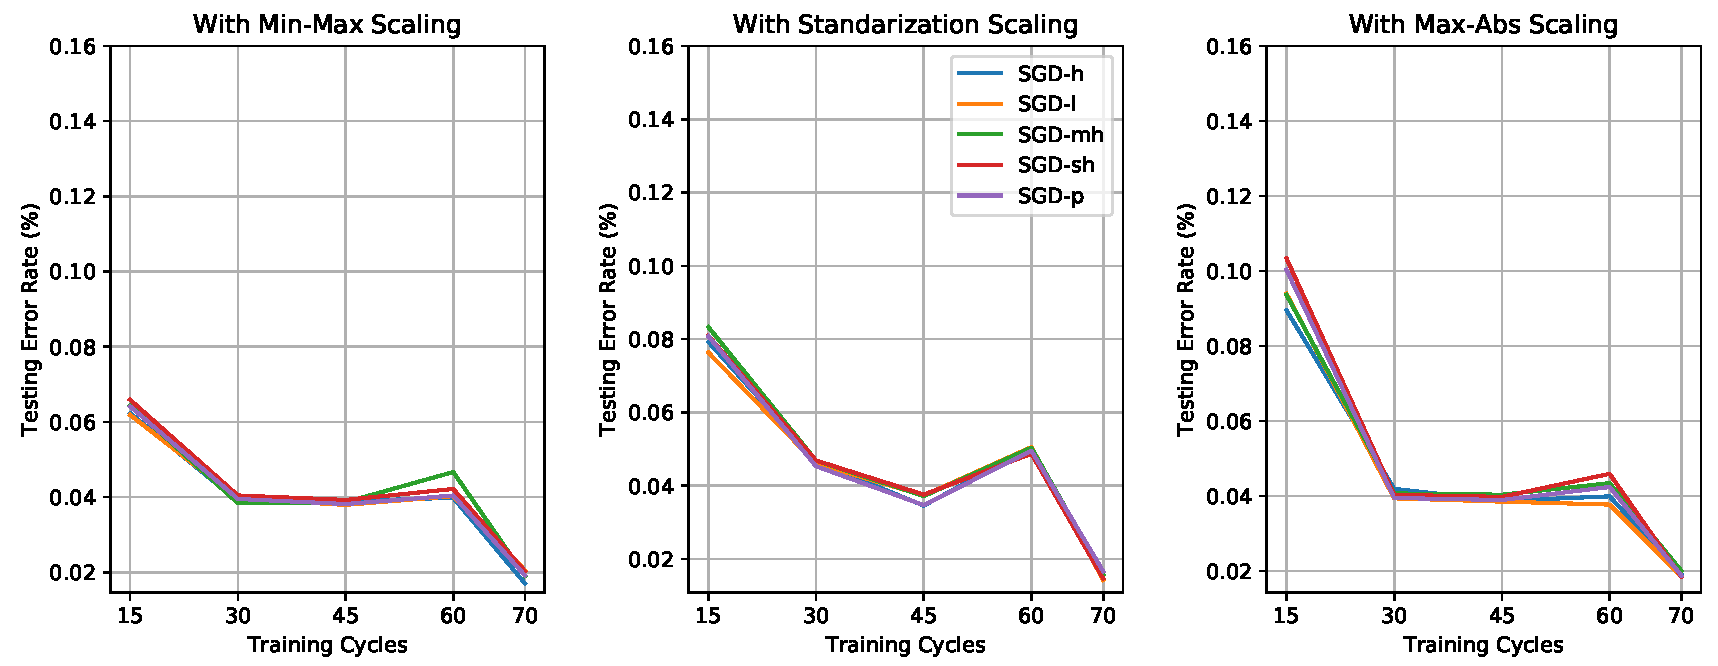
\includegraphics[keepaspectratio, width=\linewidth]{graphs/SGDClassifiersWithPenaltyL1.pdf}
	\caption{SGD instances with L1 penalty}
	\label{SGDCL1}
\end{figure}
\begin{figure}[H]
	\centering
	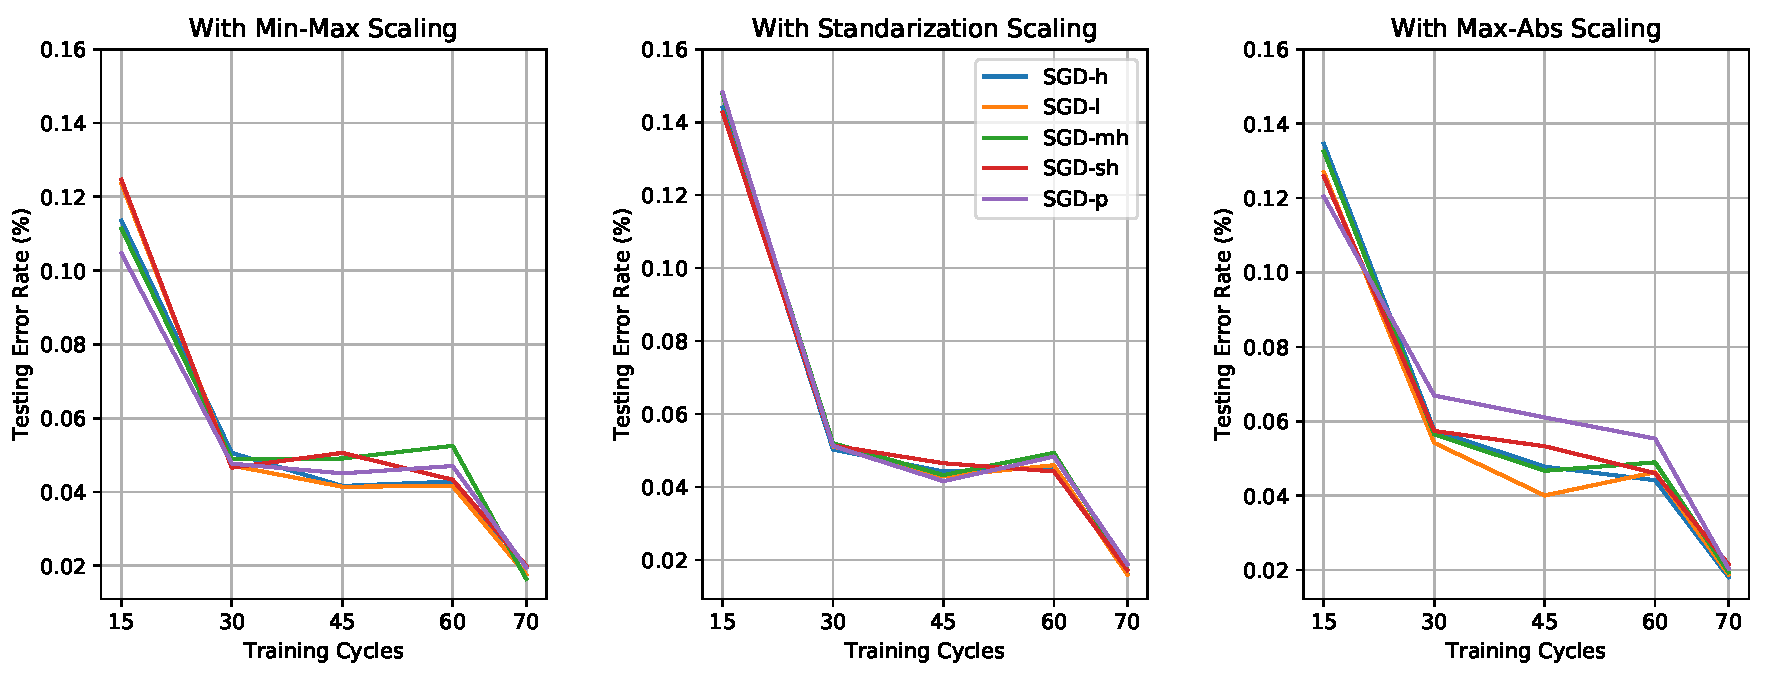
\includegraphics[keepaspectratio, width=\linewidth]{graphs/SGDClassifiersWithPenaltyL2.pdf}
	\caption{SGD instances with L2 penalty}
	\label{SGDCL2}
\end{figure}
\begin{figure}[H]
	\centering
	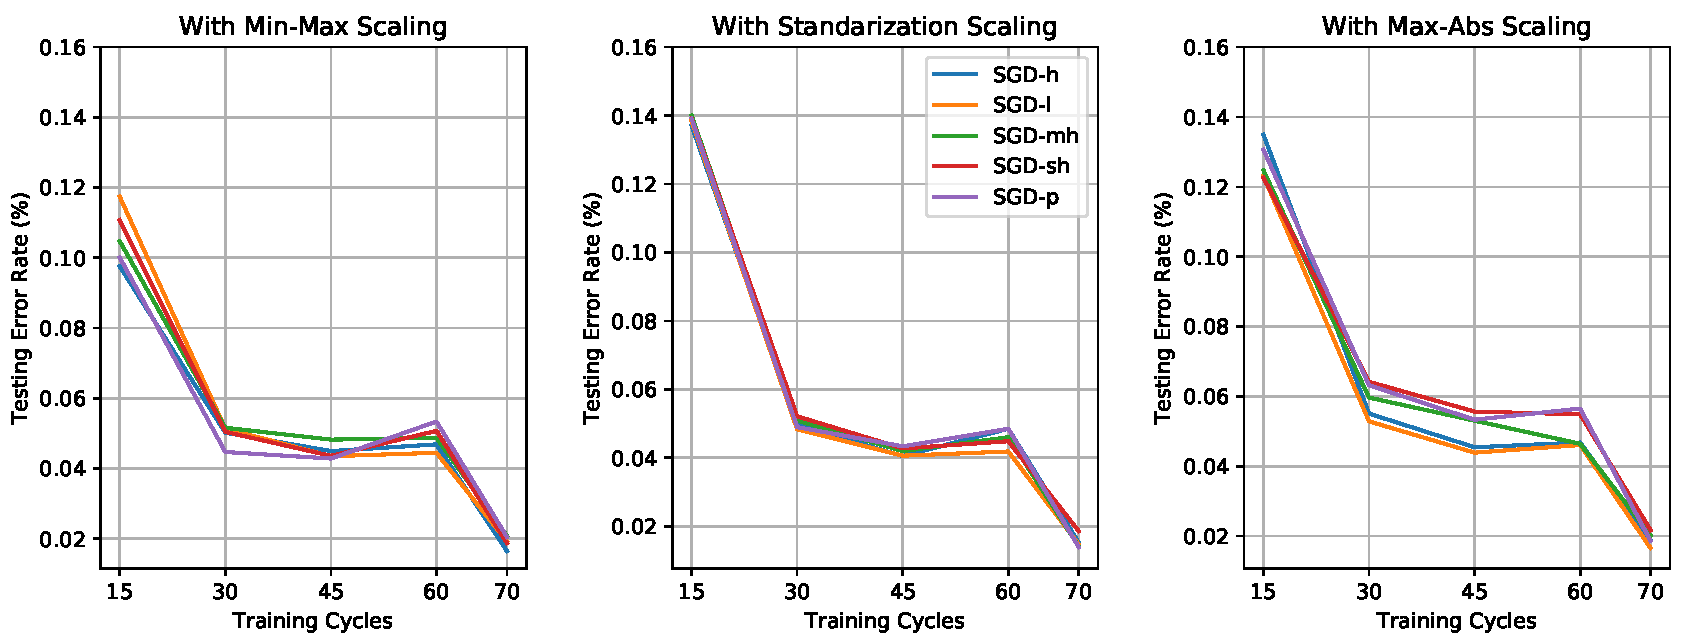
\includegraphics[keepaspectratio, width=\linewidth]{graphs/SGDClassifiersWithPenaltyElasticnet.pdf}
	\caption{SGD instances with elasticnet penalty}
	\label{SGDCElasticnet}
\end{figure}
It is clear from the figures \ref{SGDCL1}, \ref{SGDCL2} and \ref{SGDCElasticnet} that L1 penalty enabled the SGD instances to accomplish the learning goals. SGD instances achieved the learning goals with min-max and max-abs scaling algorithms. However, with min-max the testing error rate of the instances are lower compared to max-abs. In min-max, SGD-h is slightly better than other after passing 60 training cycles. Therefore, we selected SGD-h with penalty L1. Later, we used SGD-h in the model selection process to compete with the instances of Perceptron and PA, see figure \ref{Classifiers}. Listing \ref{SGDClassifiers} shows the hyperparameters of SGD instances used in this selection process.
\begin{lstlisting}[language=json, caption=Hyperparameters of SGD instances for classification, label=SGDClassifiers]
#SGD-h
SGDClassifier(loss='hinge', penalty='l1')
SGDClassifier(loss='hinge', penalty='l2')
SGDClassifier(loss='hinge', penalty='elasticnet')

#SGD-l
SGDClassifier(loss='log', penalty='l1')
SGDClassifier(loss='log', penalty='l2')
SGDClassifier(loss='log', penalty='elasticnet')

#SGD-mh
SGDClassifier(loss='modified_huber', penalty='l1')
SGDClassifier(loss='modified_huber', penalty='l2')
SGDClassifier(loss='modified_huber', penalty='elasticnet')

#SGD-sh
SGDClassifier(loss='squared_hinge', penalty='l1')
SGDClassifier(loss='squared_hinge', penalty='l2')
SGDClassifier(loss='squared_hinge', penalty='elasticnet')

#SGD-p
SGDClassifier(loss='perceptron', penalty='l1')
SGDClassifier(loss='perceptron', penalty='l2')
SGDClassifier(loss='perceptron', penalty='elasticnet')
\end{lstlisting}
\subsection{The Selection of SGD for Regression} \label{SGDRegressorsTests}
\begin{figure}[H]
	\centering
	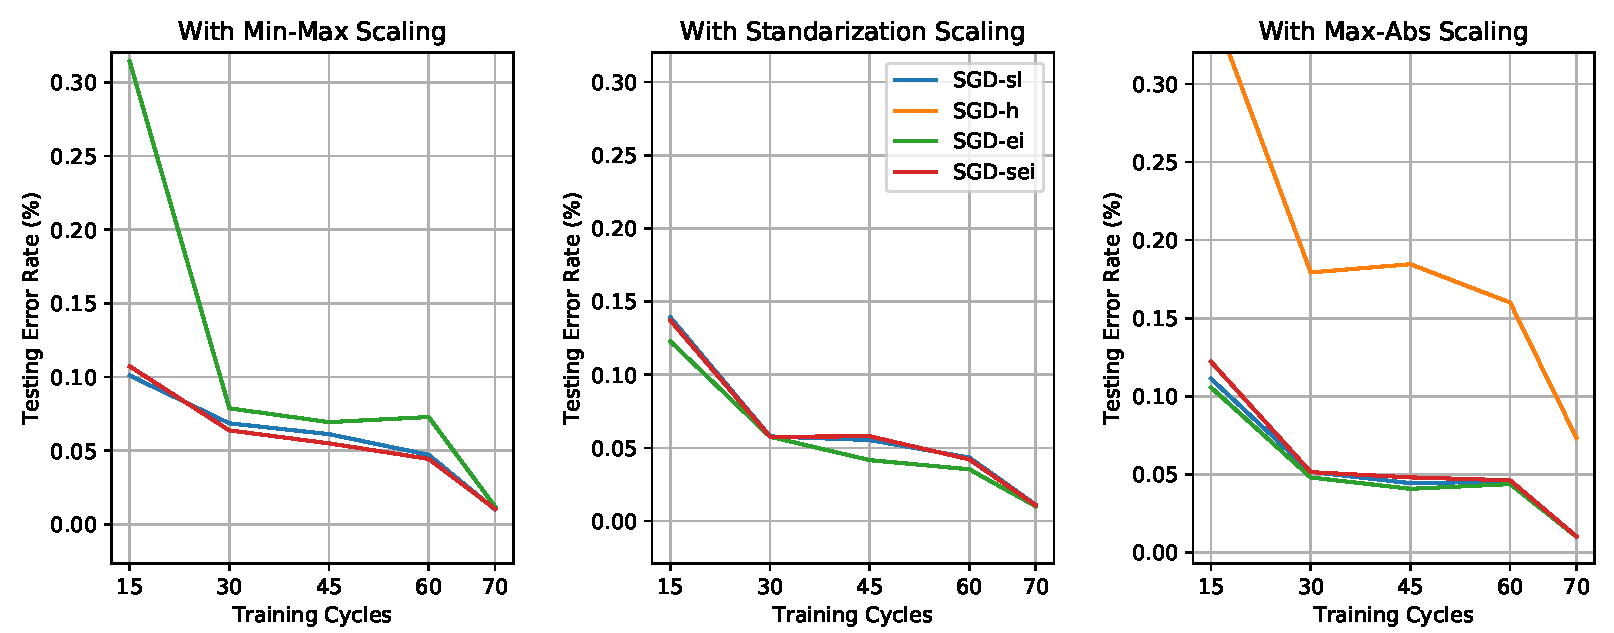
\includegraphics[keepaspectratio, width=\linewidth]{graphs/SGDRegressorsWithPenaltyL1.pdf}
	\caption{SGD instances with L1 penalty}
	\label{SGDRL1}
\end{figure}
\begin{figure}[H]
	\centering
	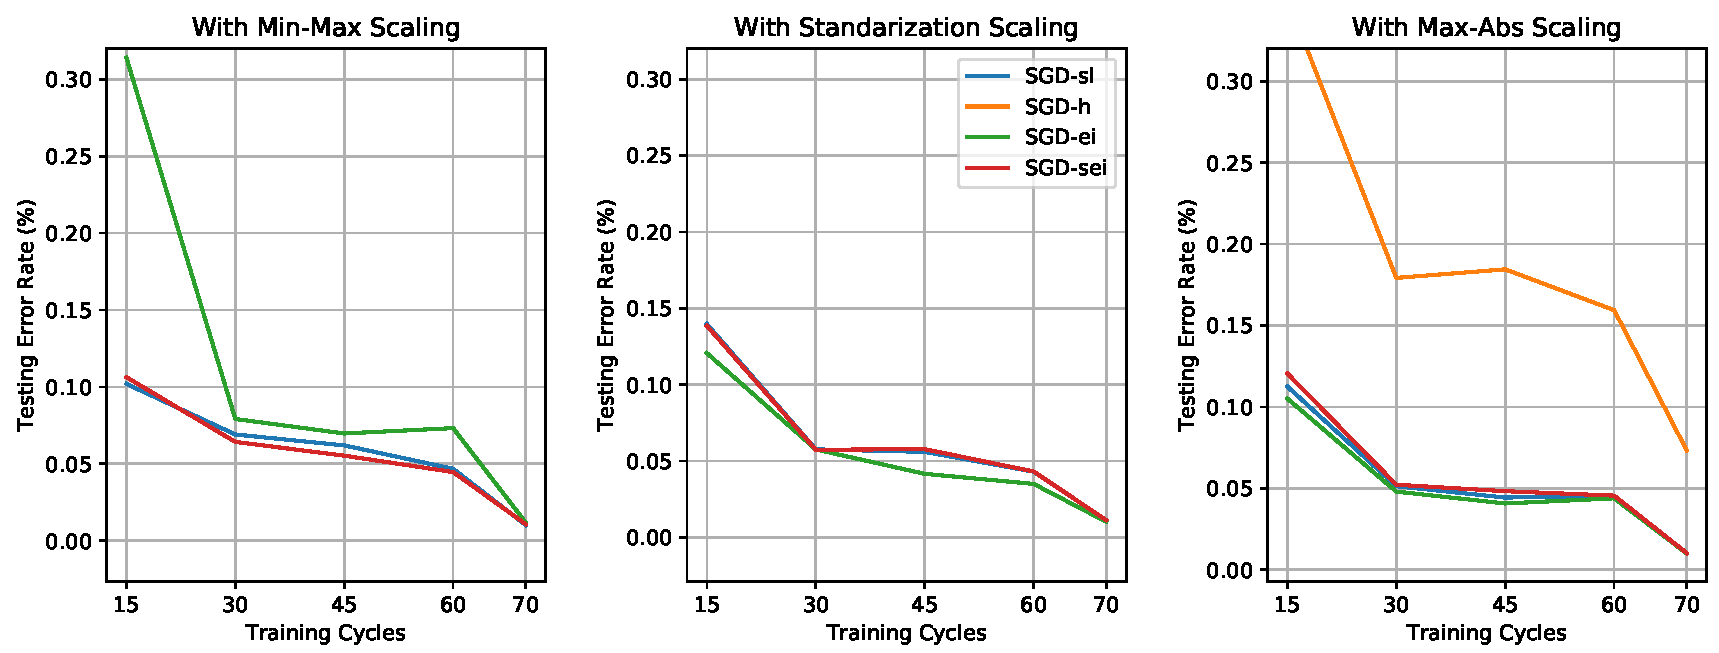
\includegraphics[keepaspectratio, width=\linewidth]{graphs/SGDRegressorsWithPenaltyL2.pdf}
	\caption{SGD instances with L2 penalty}
	\label{SGDRL2}
\end{figure}
\begin{figure}[H]
	\centering
	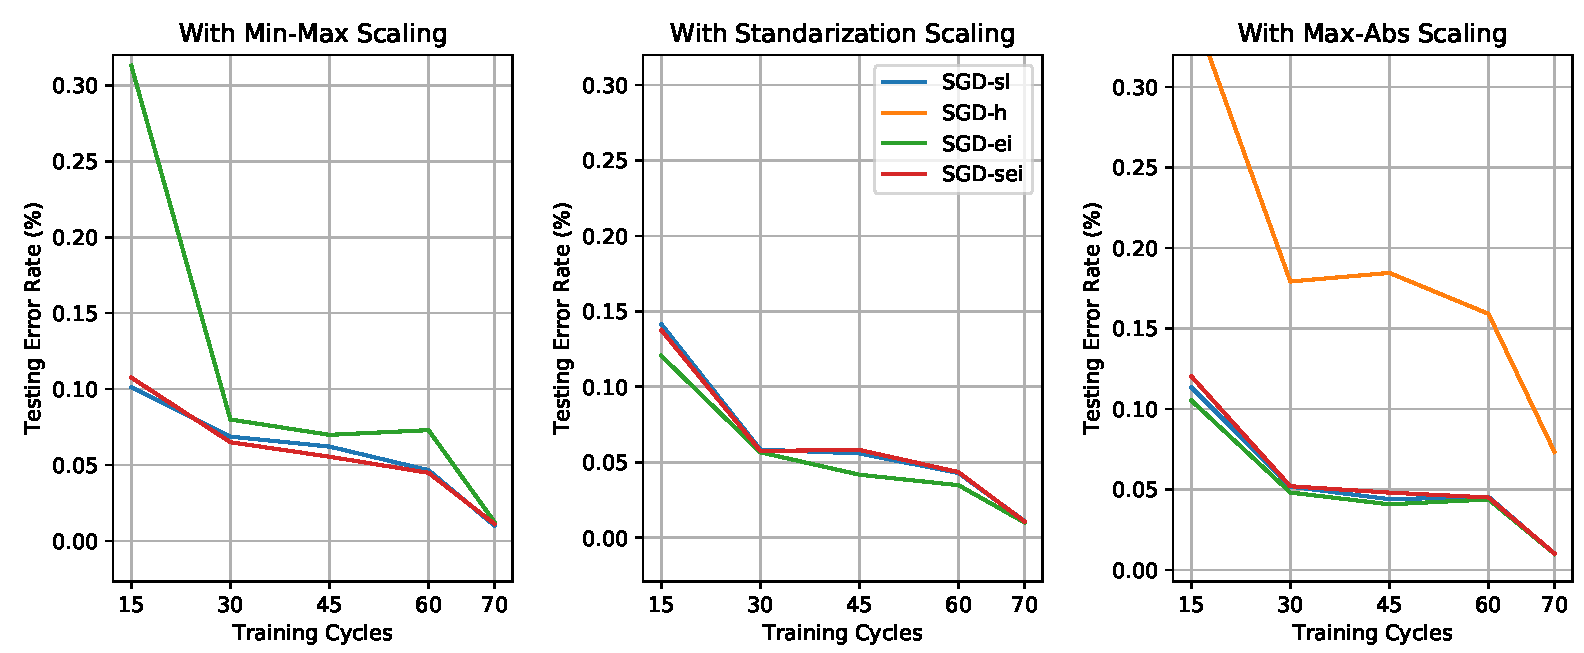
\includegraphics[keepaspectratio, width=\linewidth]{graphs/SGDRegressorsWithPenaltyElasticnet.pdf}
	\caption{SGD instances with elasticnet penalty}
	\label{SGDRElasticnet}
\end{figure}
Figures \ref{SGDRL1}, \ref{SGDRL2} and \ref{SGDRElasticnet} show that no penalty has any impact on the performance of SGD instances. The figures also show that SGD-ei achieved the learning goals with max-abs scaling algorithm. Therefore, we selected SGD-ei with default penalty, i.e., L2. Later, we used SGD-h in the model selection process to compete with the instances of PA, see figure \ref{Regressors}. Listing \ref{SGDRegressors} shows the hyperparameters of SGD instances used in this selection process.
\begin{lstlisting}[language=json, caption=Hyperparameters of SGD instances for regression, label=SGDRegressors]
#SGD-sl
SGDRegressor(loss='squared_loss', penalty='l1')
SGDRegressor(loss='squared_loss', penalty='l2')
SGDRegressor(loss='squared_loss', penalty='elasticnet')

#SGD-h
SGDRegressor(loss='huber', penalty='l1')
SGDRegressor(loss='huber', penalty='l2')
SGDRegressor(loss='huber', penalty='elasticnet')

#SGD-ei
SGDRegressor(loss='epsilon_insensitive', penalty='l1')
SGDRegressor(loss='epsilon_insensitive', penalty='l2')
SGDRegressor(loss='epsilon_insensitive', penalty='elasticnet')

#SGD-sei
SGDRegressor(loss='squared_epsilon_insensitive', penalty='l1')
SGDRegressor(loss='squared_epsilon_insensitive', penalty='l2')
SGDRegressor(loss='squared_epsilon_insensitive', penalty='elasticnet')
\end{lstlisting}
\newpage
\section{Appendix 3} \label{Hyperparameters}
In this section, we provide the hyperparameters of the learning algorithms used in the model selection process.
\begin{lstlisting}[language=json, caption=Hyperparameters of the learning algorithms for classification, label=ClassifiersSettings]
#SGD
SGDClassifier(loss='hinge', penalty='l1')

#Perceptron-I
Perceptron(penalty='l1')

#Perceptron-II
Perceptron(penalty='l2')

#Perceptron-III
Perceptron(penalty='elasticnet')

#PA-I
PassiveAggressiveClassifier(loss='hinge')

#PA-II
PassiveAggressiveClassifier(loss='squared_hinge')
\end{lstlisting}
\begin{lstlisting}[language=json, caption=Hyperparameters of the learning algorithms for regression, label=RegressorsSettings]
#SGD
SGDRegressor(loss='hinge', penalty='l1')

#PA-I
PassiveAggressiveRegressor(loss='epsilon_insensitive')

#PA-II
PassiveAggressiveRegressor(loss='squared_epsilon_insensitive')
\end{lstlisting}
\end{document}